\documentclass[conference,final]{IEEEtran}

\usepackage{latex8}
\usepackage[utf8]{inputenc}
\usepackage{url}
\usepackage{float}
\usepackage{times}    
\usepackage{listings}   
\usepackage{paralist}    
\usepackage{wrapfig}    
\usepackage[small,it]{caption}
\usepackage{multirow}
\usepackage{ifpdf}
%\usepackage{srcltx}
\usepackage{subfigure}
\usepackage{xspace}
\usepackage{keyval}  
\usepackage{color}

\definecolor{listinggray}{gray}{0.95}
\definecolor{darkgray}{gray}{0.7}
\definecolor{commentgreen}{rgb}{0, 0.4, 0}
\definecolor{darkblue}{rgb}{0, 0, 0.4}
\definecolor{middleblue}{rgb}{0, 0, 0.7}
\definecolor{darkred}{rgb}{0.4, 0, 0}
\definecolor{brown}{rgb}{0.5, 0.5, 0}

\usepackage[normalem]{ulem}
\makeatletter
\def\cyanuwave{\bgroup \markoverwith{\lower3.5\p@\hbox{\sixly \textcolor{cyan}{\char58}}}\ULon}
\def\reduwave{\bgroup \markoverwith{\lower3.5\p@\hbox{\sixly \textcolor{red}{\char58}}}\ULon}
\def\blueuwave{\bgroup \markoverwith{\lower3.5\p@\hbox{\sixly \textcolor{blue}{\char58}}}\ULon}
\font\sixly=lasy6 % does not re-load if already loaded, so no memory problem.
\makeatother

\newif\ifdraft
\drafttrue

\ifdraft
\newcommand{\onote}[1]{ {\textcolor{cyan} { (***Ole: #1) }}}
\newcommand{\terminology}[1]{ {\textcolor{red} {(Terminology used: \textbf{#1}) }}}
\newcommand{\owave}[1]{ {\cyanuwave{#1}}}
\newcommand{\jwave}[1]{ {\reduwave{#1}}}
\newcommand{\alwave}[1]{ {\blueuwave{#1}}}
\newcommand{\jhanote}[1]{ {\textcolor{red} { ***shantenu: #1 }}}
\newcommand{\alnote}[1]{ {\textcolor{blue} { ***andrel: #1 }}}
\newcommand{\amnote}[1]{ {\textcolor{blue} { ***andrem: #1 }}}
\newcommand{\smnote}[1]{ {\textcolor{brown} { ***sharath: #1 }}}
\newcommand{\msnote}[1]{ {\textcolor{cyan} { ***mark: #1 }}}
\newcommand{\note}[1]{ {\textcolor{magenta} { ***Note: #1 }}}
\else
\newcommand{\onote}[1]{}
\newcommand{\terminology}[1]{}
\newcommand{\owave}[1]{#1}
\newcommand{\jwave}[1]{#1}
\newcommand{\alnote}[1]{}
\newcommand{\amnote}[1]{}
\newcommand{\athotanote}[1]{}
\newcommand{\smnote}[1]{}
\newcommand{\jhanote}[1]{}
\newcommand{\msnote}[1]{}
\newcommand{\note}[1]{}
\fi

\newcommand{\pilot}{Pilot\xspace}
\newcommand{\pilots}{Pilots\xspace}
\newcommand{\pilotjob}{Pilot-Job\xspace}
\newcommand{\pilotjobs}{Pilot-Jobs\xspace}
\newcommand{\computeunit}{Compute Unit\xspace}
\newcommand{\computeunits}{Compute Units\xspace}
\newcommand{\cu}{CU\xspace}
\newcommand{\cus}{CUs\xspace}
\newcommand{\cs}{Compute Service\xspace}
\newcommand{\css}{Compute Services\xspace}
\newcommand{\dataunit}{Data Unit\xspace}
\newcommand{\dataunits}{Data Unit\xspace}
\newcommand{\du}{DU\xspace}
\newcommand{\dus}{DUs\xspace}
\newcommand{\pilotdata}{Pilot Data\xspace}
\newcommand{\pd}{PD\xspace}
\newcommand{\pds}{Pilot Data Service\xspace}
\newcommand{\pdss}{Pilot Data Services\xspace}
\newcommand{\su}{SU\xspace}
\newcommand{\sus}{SUs\xspace}
\newcommand{\schedulableunit}{Schedulable Unit\xspace}
\newcommand{\schedulableunits}{Schedulable Units\xspace}
\newcommand{\condorg}{Condor-G/Glide-In\xspace}

\lstdefinestyle{myListing}{
  frame=single,   
  backgroundcolor=\color{listinggray},  
  %float=t,
  language=C,       
  basicstyle=\ttfamily \footnotesize,
  breakautoindent=true,
  breaklines=true
  tabsize=2,
  captionpos=b,  
  aboveskip=0em,
  belowskip=-2em,
  %numbers=left, 
  %numberstyle=\tiny
}      

\lstdefinestyle{myPythonListing}{
  frame=single,   
  backgroundcolor=\color{listinggray},  
  %float=t,
  language=Python,       
  basicstyle=\ttfamily \footnotesize,
  breakautoindent=true,
  breaklines=true
  tabsize=2,
  captionpos=b,  
  %numbers=left, 
  %numberstyle=\tiny
}

\newcommand{\up}{\vspace*{-1em}}
\newcommand{\upp}{\vspace*{-0.5em}}
\newcommand{\numrep}{8 }
\newcommand{\samplenum}{4 }
\newcommand{\tmax}{$T_{max}$ }
\newcommand{\tc}{$T_{C}$ }
\newcommand{\tcnsp}{$T_{C}$}
\newcommand{\bj}{BigJob}

 \setlength{\parskip}{0.05ex} % 1ex plus 0.5ex minus 0.2ex}
 \setlength{\parsep}{0pt}
 %\setlength{\headsep}{0pt}
 \setlength{\topskip}{0pt}
 \setlength{\topmargin}{0pt}
 %\setlength{\topsep}{0pt}
 \setlength{\partopsep}{0pt}

% This is now the recommended way for checking for PDFLaTeX:
\usepackage{ifpdf}

%\usepackage{titlesec}
%\titlespacing{\section}{0pt}{*0}{*0}
%\titlespacing{\subsection}{0pt}{*0}{*0}
%\titlespacing{\subsubsection}{0pt}{*0}{*0}

%\newif\ifpdf
%\ifx\pdfoutput\undefined
%\pdffalse % we are not running PDFLaTeX
%\else
%\pdfoutput=1 % we are running PDFLaTeX
%\pdftrue
%\fi

\ifpdf
\usepackage[pdftex]{graphicx}
\else
\usepackage{graphicx}
\fi

% \title{Towards A Framework for Pilot-Abstractions for Production
%   Cyberinfrastructure}

%\title{P*: An Extensible Model of Pilot-Abstractions for Dynamic Execution}

% \title{P*: An Extensible Model of Pilot-Abstractions}

\title{P*: A Model of Pilot-Abstractions}


% \jhanote{Alternate title: The Tiered Resource OverlaY framework
%   (TROY): An Empirical Framework for Pilot-* Abstractions}
% 
% \jhanote{old title: TROY -- Tiered Resource Overlay Framework: Towards
%   a Framework for Pilot-Abstractions for Distributed
%   Cyberinfrastructure}


\date{}

\begin{document}

\ifpdf
\DeclareGraphicsExtensions{.pdf, .jpg, .tif}
\else
\DeclareGraphicsExtensions{.eps, .jpg}
\fi

\author{
  Andre Luckow$^{1}$, Mark Santcroos$^{2,1}$, Ole Weidner$^{4,1}$, Andre Merzky$^{1}$, Sharath Maddineni$^{1}$, Shantenu Jha$^{3,1*}$\\
  \small{\emph{$^{1}$Center for Computation \& Technology, Louisiana State University, USA}}\\
  \small{\emph{$^{2}$Bioinformatics Laboratory, Academic Medical Center, University of Amsterdam, The Netherlands}}\\
  \small{\emph{$^{3}$ Rutgers University, Piscataway, NJ 08854, USA}}\\
  \small{\emph{$^{4}$ School of Informatics, University of Edinburgh, UK }}\\
  \small{\emph{$^{*}$Contact Author: \texttt{shantenu.jha@rutgers.edu}}}\\
  \up\up\up\up }

\maketitle

\begin{abstract} 
  \up 
  % Distributed cyberinfrastructures (CI) and applications require the
  % ability to determine and utilize resource
  % selection\alnote{selection somehow does not fit} at runtime
  % (dynamically), and not just before execution (statically).
  Pilot-Jobs support effective distributed resource utilization, and 
  are arguably one of the most widely-used distributed
  computing abstractions,
  % they have been utilized on many production distributed
  % cyberinfrastructures.  they have been notable in their ability to
  %\alnote{the following sentence is just a fragement}
  as measured by the number and types of applications that use them,
  as well as the number of production distributed cyberinfrastructures
  that support them.  Not surprisingly, there are multiple, distinct
  and incompatible implementations of pilot-jobs. Often these
  implementations are strongly coupled to the distributed
  cyberinfrastructure they were originally designed for.
  Additionally, in spite of broad uptake, there does not exist a well
  defined, unifying conceptual model for pilot-jobs which can be used
  to define, compare and contrast different implementations. This
  presents a barrier to extensibility and interoperability. This paper
  is an attempt to (i) provide a minimal but complete model (P*) of
  pilot-jobs, (ii) establish the generality of the P* Model by mapping
  various existing and well known \pilotjob frameworks such as Condor
  and DIANE to P*, (iii) derive an interoperable and extensible API
  for the P* Model (Pilot-API), (iv) validate the implementation of
  the Pilot-API by concurrently using multiple {\it distinct}
  pilot-job frameworks on a distinct production distributed
  cyberinfrastructures, and (v) apply the P* model to pilot-data.

  \upp\upp\upp\up

  % (iii) introduce TROY as an implementation of this
  % model, % using SAGA, i.\,e.\ consistent
  % with its API, job-model etc.,

\end{abstract}

%\note{
% \section*{Outline}
% The primary objectives of this work are:
% \begin{enumerate}
% \item Establish the need for dynamic execution of applications -
%   distributed as well as high-end performance.
% \item We define the basic characteristics of the dynamic apps and we
%   understand the requirements of dynamic apps need to do in a
%   distributed environment.
% \item We understand the capability that must be provided by the
%   infrastructure to support these application
% \item We describe the pilot-job as a good prototype of an abstraction
%   that supports dynamic execution
% \item We define the characteristics that need to be supported by a
%   pilot-job \jhanote{Infrastructure or Application characteristics?}
%   \alnote{I think we meant application characteristics}
% \item There exist multiple PJ implementations out there but no way to
%   compare and contrast. Provide a framework to aid an understanding of
%   pilot-jobs and the ability to compare, contrast and understand
%   different pilot-jobs.  Provide both a theoretical and empirically
%   useful approach to determining which PJ to use
% \item Empirical implementation of TROY and demonstration of
%   concurrent/interoperation between equivalent but distinct Pilot-Job
%   implementation. Highlight unique feature of Troy: User extensible
%   and customizable. \jhanote{We should talk about this in light of the
%     reviews of the paper with Bishop}
% \end{enumerate}
%   Points 1-3 can go into the beginning of \S2.  Points 4 \& 5 should
%   be addressed in both introduction (see one of the \jhanote{} above),
%   as well as in the beginning of \S2. Points 6, 7 are addressed in the
%   Introduction.  }

%execution model, effectively equivalent to
%The two approaches can be viewed as different approaches to the
%dynamic resource problem.
%in one, the supply is kept fixed and the demand is changed to meet the
%supply; in the other the supply changes in response to the demand.

%For the purposes of this paper, we will focus on the latter, wherein
%the availability and utilization of resources changes.  As a
%consequence, we will not consider dynamic execution arising from
%internal application changes.  
%In other words, 


% Typically, this will involve a single ``large'' distributed
% application, that is comprised of many smaller tasks.\alnote{it
%   would be good if we could relate to our DARE use case here}

% \alnote{not sure why do we need week and strong model? Determinism and
%   distributed systems don't go together well. Also, I wouldn't claim
%   that the prob. of adv. rerv. is 1 (it might be 0.99...). PJ are more
% d  in line with the weak model. Do we say that Advance Reserv. are
%   better?}  \jhanote{Addressed.} \jhanote{OK to remove?}

% There exist two models of dynamic resource utilization, which we refer
% to as the weak (probabilistic) model of dynamic execution (DE) and the
% strong (deterministic) model of DE. In the former, there exists a
% certain probability to acquire a resource at a given instant of time;
% in the latter the probability of acquiring a resource is by definition
% is 1, but there exists a broad range of times over which this
% probability will first be 1. 

%or utilization ability.  this has the resultant effect of an
%application being dynamic, though dynamic resource execution maybe
%just one of multiple responses.

% Multiple approaches exist to support dynamic resource utilization, for
% example, advanced scheduling (without pre-emption) provides
% essentially a guarantee of resources at a sufficiently far out time
% window. 

% However, distributed applications that are able to break the coupling
% between workload management and resource assignment/scheduling have
% been successful at efficiently utilizing distributed resources,
% without the policy-level complexity of implementing advanced
% reservations.

%provide applications with a dynamic resource utilization requirements.  

% Distributed CI almost by definition is comprised of a set of resources
% that is fluctuating -- growing, shrinking, changing in load and
% capability.  The ability to utilize such a dynamic resource pool is
% thus an important attribute of any application that needs to utilize
% distributed CI efficiently; this is in contrast to a static resource
% utilization model characteristic of parallel and cluster computing.

% In addition, the evolution or internal dynamics of an application may
% vary, thereby changing the resource requirements.
% For example, different solvers, 
% adaptive algorithms and/or implementations, can also require
% applications to utilize different set/amounts of resources.
% We will define dynamic applications to have the ability to respond to
% a fluctuating resource pool, i.\,e., the set of resources utilized at
% time (T), $T=0$ is not the same as $T>0$.

\section{Introduction and Overview \upp\upp} 
\alnote{Should we consistently use the \pilotjob macro?}
\jhanote{We should definitely. What about the plural form?}
\alnote{\pilotjobs}

The seamless uptake of distributed infrastructures by scientific
applications has been limited by the availability of extensible,
pervasive and simple-to-use abstractions at multiple levels –
development, deployment and execution stages of scientific
applications~\cite{dpagrid2009}.  Even where meaningful abstractions
exist, the challenges of providing these abstractions in an
extensible, interoperable, reliable and scalable manner are
formidable.  

There remains scope for improvement in the availability of reusable
and extensible tools and implementations of abstractions that can
support multiple applications and are usable on different
infrastructures.  The lack of appropriate implementations has in fact
resulted in “one-off” solutions that address challenges in a highly
customized and non-reusable manner.  Tools and implementations are
often highly dependent on and tuned to a specific execution
environment, further impacting portability, reusability and
extensibility.  Performance, semantic and interface compatibility are
certainly barriers, but so is the lack of a common architecture and
framework upon which to develop similar tools is also a barrier.


%reinforces the fragmentation~\cite{dpa_surveypaper}.
% there remains, scope for improvement in both the range and number of
% supported abstractions and the type of infrastructure over which such
% abstractions are made available.

This state of affairs is exceptionally well captured in the state of
abstractions provided by pilot-jobs -- which have been one of the most
successful abstractions in distributed computing. Distributed
cyberinfrastructure is by definition comprised of a set of resources
that is fluctuating -- growing, shrinking, changing in load and
capability; this is in contrast to a static resource utilization model
traditionally a characteristic of parallel and cluster computing.  The
ability to utilize a dynamic resource pool is thus an important
attribute of any application that needs to utilize distributed CI
efficiently. \emph{Pilot-jobs (PJ)} provide a very effective
abstraction for dynamic execution and in particular for dynamic
execution and resource usage in a distributed context, as consequence
of providing a simple approach for decoupling workload management and
resource assignment/scheduling.

The fundamental reason for the success of the PJ abstraction is that
PJ liberate applications/users from the challenging requirement of
mapping specific tasks onto explicit heterogeneous and dynamic
resource pool.  PJ also thus shields application from having to
load-balance tasks across such resources.  The pilot-job abstraction
is also a promising route to address additional, as well as specific
requirements of distributed scientific
applications~\cite{ko-efficient,DBLP:conf/hpdc/KimHMAJ10}.

A variety of PJ frameworks have emerged:
Condor-G/Glide-in~\cite{condor-g} , SWIFT~\cite{Wilde2011},
DIANE~\cite{Moscicki:908910}, DIRAC~\cite{1742-6596-219-6-062049},
PanDA~\cite{1742-6596-219-6-062041}, ToPoS~\cite{topos},
Nimrod/G~\cite{10.1109/HPC.2000.846563}, Falkon~\cite{1362680} and
MyCluster~\cite{1652061} to name a few. Although they are all, for the
most parts functionally equivalent -- they support the decoupling of
workload submission from resource assignment -- it is often impossible
to use them interoperably or even just to compare them functionally or
qualitatively.

%Where effective abstractions exist a problem in the 
%The general problem applies to the specific situation of pilot-jobs.

%Different projects and users have rolled-out their own PJ
%abstractions.  

The fact that users have voted with their feet for PJs reinforces that
the PJ abstraction is both a useful and correct abstraction for
distributed CI; the fact that it has become an ``unregulated cottage
industry'' reaffirms the lack of common nomenclature, integration,
interoperability and extension, and barriers to extensibility and
interoperabilty as a consequence.  The situation is reminiscent of the
proliferation of functionally similar yet incompatible workflow
systems, where in spite of significant a posteriori effort on workflow
system extensibility and interoperability (thus providing post-facto
justification of its needs), these objectives remains difficult if not
infeasible.


% Also, maybe interoperability isnt what is desired, but reusability
% and or ease of customisation.  Talk about analogy with workflow
% systems.  Interestingly there exist many implementations of the PJ
% abstraction, wherein d

% Interestingly there exist many implementations of the PJ abstraction,
% wherein different projects and users have rolled-out their own. The
% fact that users have voted with their feet for PJs reinforces that the
% Pilot-Job is both a useful and correct abstraction for distributed CI;
% the fact that it has become an ``unregulated cottage industry''
% reaffirms the lack of common nomenclature, integration,
% interoperability and extension.



Our objective is to provide a minimal, but complete model -- hence
referred to as the P* Model, for the pilot-job abstraction.  The P*
Model provides a conceptual basis to compare and contrast different
pilot-job implementations, which to the best of our knowledge, is the
first such attempt.

% In \S{III} we introduce TROY -- A Tiered Resource OverlaY -- as an
% implementation of the P* Model. TROY provides an API for the P* Model
% and exposes the semantics of PJ frameworks; TROY also has a runtime
% system that enables it to work with different middleware on
% heterogeneous distributed platforms.

% Implementations of PJ frameworks, such as BigJob and DIANE, are
% integrated into TROY via an adaptor mechanism; we posit that the TROY
% framework and API can be used for most, if not all PJ frameworks.

We present the P* Model in \S{II}. The P* Model captures the essence
of most, if not all existing PJ frameworks. In \S{III} we validate
this claim by analyzing several well-known PJ frameworks
(Condor-G/Glide-in, DIANE, Swift-Coaster) within the framework
provided by the P* Model.

%Before validating this claim with empirical evidence

% \S{V} we present and validate

\S{IV} of this paper introduces and describe the Pilot-API; and we
discuss how BigJob, Condor-G~\cite{condor-g} and
DIANE~\cite{Moscicki:908910} -- existing and widely used pilot-job
frameworks, can be used through the Pilot-API.  \S{V} outlines the
experiments and performance measurements used to characterize the
workings of the Pilot-API and to demonstrate interoperability across
middleware, platform and different PJ frameworks.  To further
substantiate the impact of P*, we will demonstrate interoperability
between different PJ frameworks -- BigJob and DIANE. We believe this
is also the first demonstration of interoperation of different
pilot-job implementations.

After validating the P* Model -- as measured by extensibility and
interoperability, we investigate generalizations to the base P* Model
in \ \S\ref{sec:pilot-data}.  A natural and logical extension of the
P* Model, arises from the need to extend it to include data in
addition to computational tasks.  This leads to analogous abstraction
to the pilot-job: the \emph{\pilotdata (PD)} abstraction.  The
potentially consistent treatment of data and compute, suggests
symmetrical compute and data elements in the P* model; thus we refer
to this model as the P* model ("P-star").

The impact and validation of this paper lies in the practical
implications of our work, which is also partly motivated by the
status of the usage and availability of the pilot abstraction
vis-\`{a}-vis the current landscape of distributed applications and
cyberinfrastructure.  Pilot-Jobs are used on every major national and
international distributed CI, including NSF XSEDE, NSF/DOE Open
Science Grid, EU EGI amongst others. Collectively pilot-jobs support
hundreds of thousands if not millions of tasks every day.  As we will
show, the Pilot-API provides a single uniform API to PJ-frameworks
thus providing for the first time... removing barriers to...
 


\section{P* Model: An Abstract Model for Pilot-Abstractions\upp\upp}
\label{sec:pilot-model}

To provide a common analytical framework to understand the most
commonly used pilot-jobs, we present the P* model of
pilot-abstractions. The P* model is derived from an analysis of many
pilot-job implementations; based upon this analysis, we first present
the common {\it elements} of the P* model, followed by a description
of the {\it characteristics} that determine the interaction of these
elements and the overall functioning of a pilot-job framework that is
consistent with the P* model.

%All pilot-job frameworks (whether they adhere rigorously to the P*
%model or not), have these {\it elements}, but differ in {\it
%  characteristics}.
%specific attributes \alnote{What would be an attribute in this
%  context?} and

% Further, we will show that
% these elements and interactions can be used to describe a pilot-data
% model.
 
Before we proceed to discuss the P* Model, it is important to
emphasize that there exist a plethora of terms --- abstraction, model,
framework, and implementation, that are overloaded and overlapping,
and often even used inconsistently in the literature; thus we
establish their context and usage in this paper.

\emph{Terms and Usage:} The \emph{ abstraction} of a pilot-job
generalizes the reoccuring concept of utilizing a placeholder job as a
container for a set of compute tasks; instances of that placeholder
job are commonly referred to as \emph{pilot-jobs} or
\emph{pilots}. The P* \emph{model} provides a % specific,
comprehensive description of pilot-job abstractions based on a set of
identified elements and their interactions. The P* model can be used
as a {\it conceptual model}, for analyzing different implementations
of the pilot-job abstraction. \alnote{Can the next sentence moved more
  toward PJ framework?} \jhanote{Yes, please do so} It is important to
distinguish P* which provides a conceptual (abstract) model from an
implementation of the P* model; the \emph{Pilot-API} exposes a sub-set
of the P* elements and characteristics to applications. Finally, a
\emph{pilot-job framework} refers to a specific instance of a
pilot-job implementation and associated infrastructure that provides
the complete pilot-job functionality (e.\,g.\ Condor-G and
DIANE). 

%\alnote{The next sentence is not really helpful - we also not really
%  using the term PJ system in the rest of the paper:} The term
%"pilot-job system" could have been used as well, but past experience
%shows that even with ``system'', there remains scope for confusion
%between the pilot-job itself and associated infrastructure (e.g, the
%literature abounds with inconsistent usage of the term ``workflow
%systems'').

% \jhanote{\emph{Other Terms:} Resource-Manager and agent..}
% \jhanote{This could be a good place to describe (not define) an 

\begin{figure}[t]
    \centering\up
    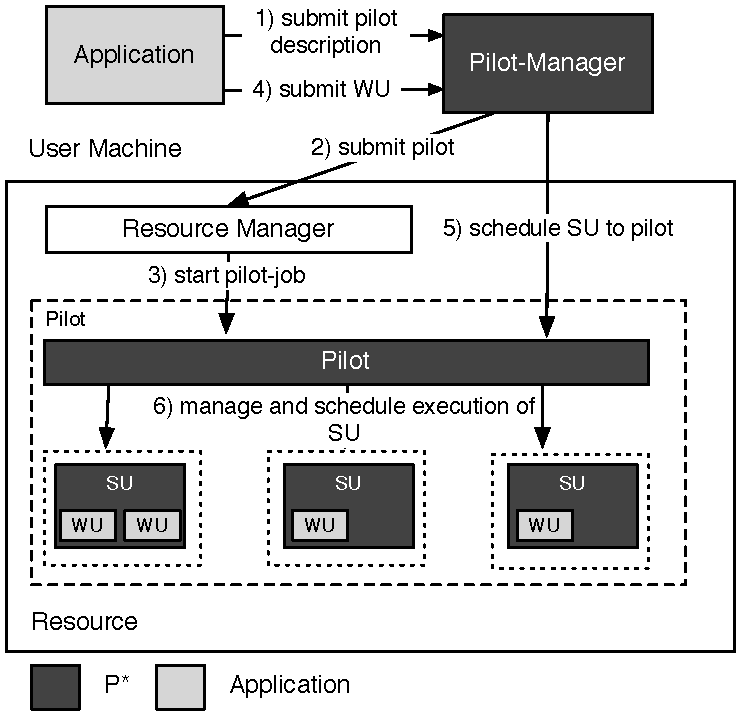
\includegraphics[width=0.43\textwidth]{figures/pstar_model_single.pdf}
    \caption{ \textbf{P* Model: Elements, Characteristics and
        Interactions:} The manager has two functions: it manages 1)
      Pilots (step 1-3) and 2) the execution of \cus. After a \cu is
      submitted to the manager, it transitions to an \su, which is
      scheduled to a \pilot by the PM. The \pilot then schedules the
      \su to an available resource. \alnote{fix caption!}  \upp\upp}
    \label{fig:figures_pstar}
\end{figure}




%\input{sectionII_comments}

\noindent 
\subsection{Elements of the P* Model \upp\upp}
\noindent This sub-section defines the elements of the P* model:

\alnote{use pilot NOT pilot-job}
\begin{compactitem}
\item \textbf{\pilot \ (Pilot-Compute):} The pilot is the
  entity that actually gets submitted and scheduled on a resource
  using the resource's RM system. The PJ provides application (user)
  level control and management of the set of allocated resources.

  % and is responsible for the execution of \alwave{SUs/tasks}
  % onto the resource.

  % \alnote{\textbf{The RM assigns a slice of the Resource to the
  %     pilot -- that pilot then acts as RM for that resource slice.}
  %   I think simply equating a pilot with a RM is bit too
  %   simplistic. In a sense it is a application-level resource
  %   manger. Not sure what to do}

\item \textbf{\computeunit \ (\cu):} A \cu \ encapsulates a self-contained
  piece of work (a task) specified by the application that is
  submitted to the pilot-job framework.  There is no intrinsic notion
  of resource associated with a \cu.

\item \textbf{Scheduling Unit (SU):} SUs are the units of scheduling
  used internal to the P* model, i.e., an SU is not known by or
  visible to an application. Once a \cu has been
  passed into the control of the \pilotjob framework, it is assigned
  to an SU.
  % An SU is created after the submission of
  %   a \cu, i.\,e.\ once a \cu \ has been passed into the control of the
  %   pilot-job framework. 
%  \jhanote{Could we say: Once a \cu has been
%    passed into the control of the pilot-job framework, it is assigned
%    to an SU} \alnote{sounds good. done.}

\item \textbf{Pilot-Manager (PM):} The PM is responsible for (i)
  orchestrating the interaction between the pilots as well as the
  different components of the P* model (\cus, \sus) and (ii) decisions
  related to internal resource assignment (once resources have been
  acquired by the pilot-job).  For example, an SU can consists of one
  or more \cus. Further, \cus and \sus can be combined and aggregated;
  the PM determines how to group them, when \sus are scheduled and
  executed on a resource via the \pilot, as well as how many resources
  to assign to an SU.

% the different characteristics of the P* model. It
%   facilitates the coordination between the different P* elements,
%   i.\,e.\ the pilots, \cus and SUs. 
% A PM can e.\,g.\ manage solely one
%   or multiple pilots.

%   For example, the PM has the flexibility to combine and schedule \cus,
%   e.\,g.\ it can determine when a \cu is run and what as well as how
%   many resources it will receive.

\end{compactitem}

% The application itself is not strictly part of the core P* Model.
% The term application generally refers to the upper layer of the
% stack.

An application kernel is the actual binary that gets executed.  The
application utilizes a PJ framework to execute multiple instances of
an application kernel (an ensemble) or alternatively instances of
multiple different application kernels (a workflow).  To execute an
application kernel, an application must define a \cu \ specifying the
application kernel as well as other parameters. This \cu \ is then
submitted to the pilot-manager (as an entry point to the
pilot-framework), where it transitions to an SU. The PM is then
responsible for scheduling the SU onto a pilot and then onto a
physical resource.  As we will see in \S{IV}, the above elements can
be mapped to specific entities in many pilot-jobs in existence and
use; often more than one logical element may be rolled into a specific
entity in a pilot-job.

% \textbf{Diane Definition of Terms: } The computation consists of
% many worker processes which communicate with one master process (the
% worker processes do not need to share the filesystem nor
% memory). The ensemble of computation is called a run and it consists
% of many tasks which may be executed in parallel. A task is defined
% as a set of parameters which are produced by the RunMaster (running
% on a master node) and consumed by the WorkerAgent (running on a
% worker node).
% 
% from 
% 
% DIANE assumes the master-worker computing model (Fig.
% 1). Client sends job parameters to the Planner which partitions
% the job into smaller tasks executed by the Workers. Integrator
% is responsible for merging the results of task execution and
% sending the final job outcome to the Client.


\subsection{Characteristics of P* Model:\upp\upp}
\label{sec:p_star_elements}

%\jhanote{Why not have Binding as the first characteristics?}

% To understand % the degrees of freedom that any specific pilot-job
% % implementation must constraint as well as
% the functioning of
% pilot-jobs implementation, 
%These characteristics are integral components of the P* Model, in
% Further, these properties are important for the implementation of
% P*.  list several characteristics.
% The way the coordination between the different elements
% is handled is required to understand a PJ implementation.
 
We propose a set of fundamental properties/characteristics that
describe the interactions between the elements, and thus aid in the
description of P* model.

% \alnote{ok} \jhanote{One strategy could be to not define the different
%   types, but just list/enumerate? Akin to Communication. i.e. explain
%   what coordination is for, what is being coordinated, how (the 3
%   types)}

\textbf{Coordination:} The coordination characteristics describes how
various elements of the P* Model, i.\,e.\ the PM, the pilot, the \cus
and the SUs, interact. A common coordination pattern is master/worker
(M/W): the PM represents the master process that controls a set of
worker processes, the pilots. The point of decision making is the
master process. In addition to the \emph{centralized} M/W, M/W can
also be deployed \emph{hierarchically}.  Alternatively, coordination
between the elements, in particular the pilots, can be performed so as
to be \emph{decentralized}, i.\,e.\ without central decision making
point.

%\input{sectionIII-comments}

\textbf{Communication:} The communication characteristics describes the
mechanisms for data exchange between the elements of the P* Model:
e.\,g.\ messages (point-to-point, all-to-all, one-to-all, all-to-one,
or group-to-group), streams (potentially unicast or multicast),
publish/subscribe messaging or shared data spaces.
		
\textbf{Scheduling:} The scheduling characteristics describes the
process of mapping a SU to resources via a pilot and potential
multiple levels of scheduling. Scheduling has a spatial component
(which SU is executed on which pilot?) but also a temporal component
(when to bind?). The different scheduling decisions that need to be
made are representative of multi-level scheduling decisions that are
often required in distributed environments.  For example, when should
a SU be bound to a pilot?  An SU can be bound to a pilot either before
the pilot has in turn been scheduled ({\it early} binding), whereas
{\it late} binding occurs if the SU is bound after the pilot has been
scheduled.  In general, there are multiple-levels at which scheduling
decisions, i.e., resource selection and binding, are made.

The term {\it agent}, although not a part of the P* Model, finds
mention when discussing implementations. For the purposes of this
paper, an agent refers to a ``proxy process'' 
% that either % inside the % pilot-job framework
that has some decision making capability, and could aid the
implementation of one or more of the characteristics of the P* Model
-- coordination, communication, scheduling, within a pilot-job
framework.  These agents can be used to enforce, a set of
(user-defined) policies (e.g.  resource capabilities, data/compute
affinities, etc.) and heuristics.

\subsection{Putting it all together} 
Figure~\ref{fig:figures_pstar}
illustrates the interactions between the elements of the P* model. In
the first step the application specifies the capabilities of the
resources required using a pilot-job description (step 1). The PM then
submits the necessary number of pilots in order to fulfill the
resource requirements of the application (step~2). Each pilot is
queued at the resource manager, which is responsible for starting the
pilot (step~3). There can be variations of this flow: while in the
described model, the application defines the required resources, the
PM could also decide based on the submitted \cu \ workload whether and
when it submits new pilots.

%\jhanote{What about the Resource Manager? Is it part of the resource}

The application can submit \cus to the PM at any time (step~4). A
submitted \cu \ becomes an SU, i.\,e.\ the PM is now in control of
it. In the simplest case one \cu \ corresponds to one SU; however,
SUs can be combined and aggregated to optimize throughputs and
response times. Commonly, a hierarchical M/W model for coordination
is used internally: the PM uses M/W to coordinate a set of pilots,
the pilot itself functions as manager for the execution of the
assigned SUs.

The PM is responsible for selecting a pilot on which an SU is executed
(step 5). Once a SU has been scheduled to a pilot, the pilot decides
when and on which physical resource the SU is executed. \jhanote{Isn't
  the pilot already bound to a specific resource? Or isn't the pilot
  bound to a resource and thereby the SU bound to a resource
  indirectly, and not directly?}  \alnote{Yes, the pilot is bound to a
  specific resource set, assigning a SU to a pilot means that it can
  be executed somewhere on this resource set. The pilot decides on
  which node a SU is run. There can be trivial cases, e.g. DIANE where
  this decision making does not exist: 1 worker agent == 1 core == 1
  task. Should we make this more explicit?} \jhanote{Yes -- we
  could/should make more explicit the fact that pilot is already bound
  to a resources and assigning a SU to a pilot means it can be
  executed anywhere on this resource set.} Further, the pilot also
manages the subsequent execution of the SU (step~6).  Again there can
be variations of this flow. The above description presents a typical
example of the inner working of a PJ framework, but alternative
implementation of the P* characteristics are possible. PJ frameworks
with decentralized decision making e.\,g.\ often utilize autonomic
agents that accepts respectively pull SUs according to a set of
defined policies.


\section{Pilot-Job Frameworks\upp\upp}

% \note{OW says: we have this obsession with the term 'framework', but
%   not everything is a framework, e.g., while BigJob and DIANE somewhat
%   resemble a framework, I do not see how Condor can qualify as one.\\
%   For now, I changed the title to 'systems'. If there are no
%   objections, I will make this consistent throughout the
%   text}\alnote{I think we should keep frameworks, I do not see why
%   Condor is not a framework - we also would break consistency with our
%   terms and definitions in section II.}\note{OW says: "In computer
%   programming, a software framework is an abstraction in which
%   software providing generic functionality can be selectively changed
%   by user code, thus providing application specific software." This is
%   definetely not the case for Condor and not really for BigJob. DIANE
%   somewhat resembles a framework.}  \note{OW says: What if we call it
%   Pilot-Job Implementations}

As more applications take advantage of dynamic execution, the
Pilot-Job concept has grown in popularity and has been extensively
researched and implemented for different usage scenarios and
infrastructure. There is a variety of PJ implementations:
Condor-G/Glide-in~\cite{condor-g}
, SWIFT~\cite{Wilde2011},
DIANE~\cite{Moscicki:908910}, DIRAC~\cite{1742-6596-219-6-062049},
PanDA~\cite{1742-6596-219-6-062041}, ToPoS~\cite{topos},
Nimrod/G~\cite{10.1109/HPC.2000.846563}, Falkon~\cite{1362680} and
MyCluster~\cite{1652061} to name a few. The aim of this section is to
show that our P* Model can be used to explain/understand some of these
PJ frameworks. In particular we focus on BigJob, DIANE and Condor-G/Glide-in.

\alnote{Is this a place to to describe ``native'' PJs for different 
infrastructures}

%\jhanote{The aim of this section is to provide a conceptual validation
%  of the P* model by describing/explaining the most commonly used
%  PJ-frameworks and showing how the individual PJ-frameworks map to
%  the P* model, i.e., can be explained by the P* model}


\upp
\subsection{Condor-G/Glide-in\upp\upp}

Condor-G pioneered the Pilot-Job concept~\cite{condor-g}. The pilot is
actually a complete Condor pool that is started using the Globus
service of a resource. This mechanism is referred to as Condor
Glide-In. Subsequently, jobs can be submitted to this Glide-In pool
using the standard Condor tools and APIs. Condor utilizes a
master/worker coordination model. The PJ manager is referred to as the
Condor Central Manager. The functionality of the Central Manager is
provided by several daemons: the condor\_master that is generally
responsible for managing all daemons on a machine, the
condor\_collector which collects resource information, the
condor\_negotiator that does the matchmaking and the condor\_schedd
that is responsible for managing the binding and scheduling
process. Condor generally does not differentiate between workload,
i.\,e.\ \cu, and schedulable entity, i.\,e.\ SU. Both entities are
referred to as job. However, it supports late binding, i.\,e.\
resources a job is submitted to must generally not be available at
submission time. The scheduler matches the capabilities required by a
\cu to the available resources. This process is referred to as
matchmaking. Further, a priority-based scheduler is used. For
communication between the identified elements Condor utilizes
point-to-point messaging using a binary protocol on top of TCP.

Different fault tolerance mechanisms, such as automatic retries, are
supported.  Further, Condor supports different security mechanisms:
for authentication it integrates both with local account management
systems (such as Kerberos) as well as grid authentication systems such
as GIS. Communication traffic can be encrypted.

\noindent \textbf{PJ Exposure on Open Science Grid:} Describe 
how PJs are hidden via Glide-In WMS.


\subsection{BigJob: A SAGA-based Pilot-Job Framework\upp\upp}
\label{sec:bigjob_description}
%\terminology{BigJob (BJ) , BigJob-SAGA, BJ implementation, BJ-SAGA, BJ
%  flavors, Amazon EC2, Microsoft Azure, BJ with a Condor Glide-In
%  based backend, BigJob Manager, BigJob agent component, BigJob
%  framework, BigJob pool, extensible scheduler, }


% \jhanote{MUST provide SAGA URL for updated BigJob API and
%   documentation}

% \jhanote{Alternative title: ``BigJob: TROY Pilot-Job'' ?}

% \jhanote{It is CRITICAL to explain why we need to expose the details
%   of multiple atomic BigJobs to the end-user? Remember part of the
%   whole idea of the exercise is, (i) theory: to provide a framework
%   for understanding any differences, (ii) practice: make all these
%   differences go away from the end user!}  \alnote{Since we were not
%   sure about the term ``atomic'', we could also use base bigjob, or
%   core bigjob}



   % 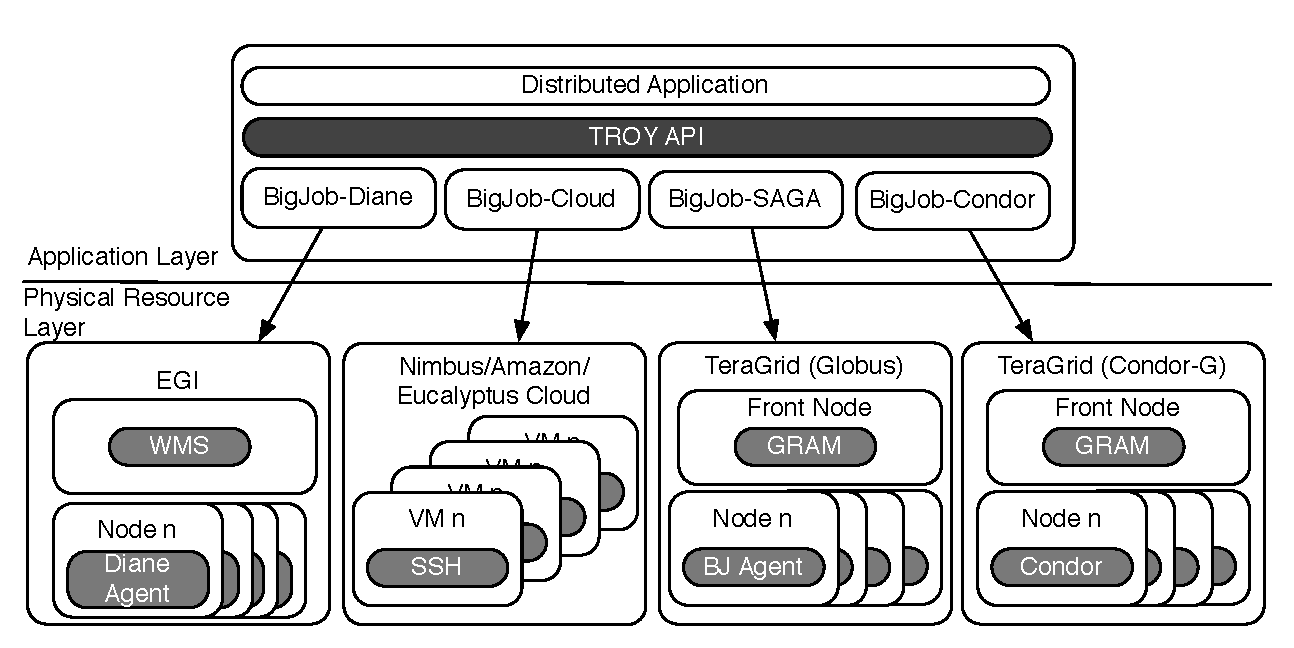
\includegraphics[width=0.3\textwidth]{figures/distributed_pilot_job.pdf}
    % 	\caption{SAGA-based TROY Implementation - BigJob}
    % 	\label{fig:figures_distributed_pilot_job}
    % 	\end{figure}


% General overview of BJ implementations & P* model
%PJ implementations in TROY are called BigJob (BJ)~\cite{bigjob_web}.

BigJob (BJ)~\cite{bigjob_web,saga_bigjob_condor_cloud} is a SAGA-based PJ
framework. BJ has been designed to be general-purpose and extensible. While BJ
has been originally built for HPC infrastructures, such as XSEDE and FutureGrid,
it is generally also usable in other environments. This extensibility mainly
arises from the usage of SAGA as a common API for accessing distributed
resources. SAGA~\cite{saga_url,ogf-gfd-90} provides a simple, POSIX-style API to
the most common grid functions at a sufficiently high-level of abstraction so as
to be independent of the diverse and dynamic grid environments.
By relying on SAGA, BJ is able to run on Globus resources prevailing in HPC
environments, as well as on Cloud resources (such as Amazon EC2 and FutureGrid)
and Condor backends.

% \jhanote{we'll have to unfortunately describe saga briefly in order to
%   make saga-based clear/obvious}\alnote{ok, moved a sentence from
%   Pilot-API section up front.}

\begin{figure}[t]
	\upp\upp\upp\upp
	\centering
	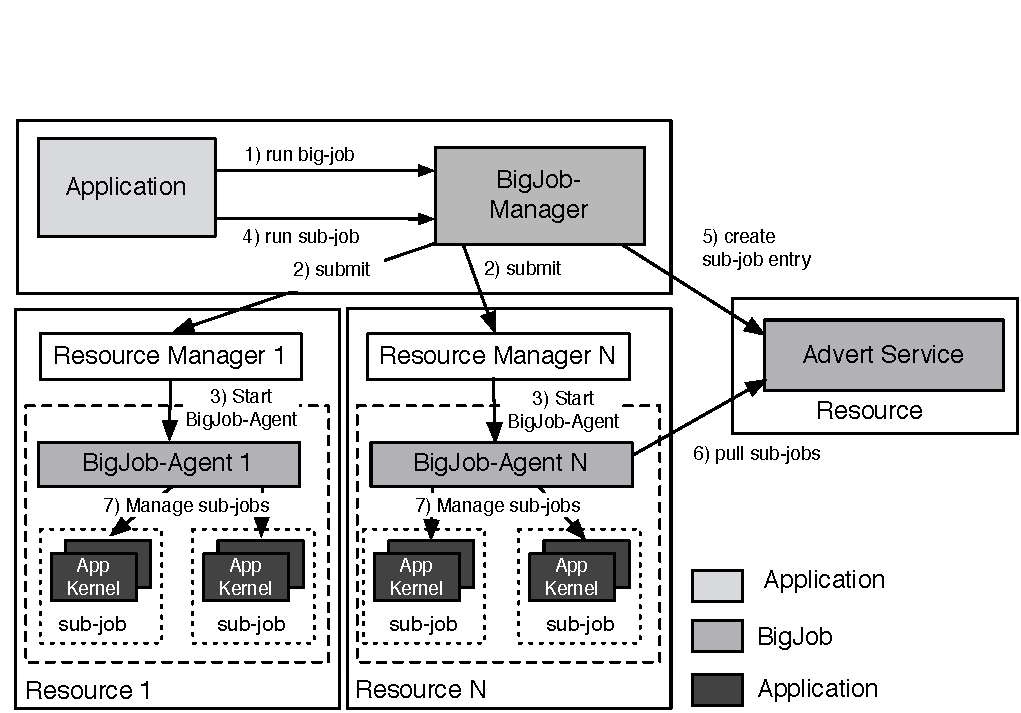
\includegraphics[width=0.45\textwidth]{figures/re_bigjob_interactions.pdf}
	\caption{\textbf{BigJob Architecture and Mapping to P*:} The
          BJ architecture resembles many elements of the P* model. The
          BigJob-Manager is the central Pilot-Manager, which
          orchestrates a set of pilots. Each pilot is represented by a
          decentral component referred to as the BigJob-Agent. Sub-job
          -- the \cus -- are submitted via the PM. \cus are mapped 1:1
          to \sus. \jhanote{Andre, I notice application occurs twice
            in the box/labels on the bottom right.. please fix}}
	\label{fig:figures_re_bigjob_interactions}
	\upp\upp \upp
\end{figure}


Figure~\ref{fig:figures_re_bigjob_interactions} illustrates the
architecture of BJ and its mapping to P*. The architecture reflects
all P* elements: The BJ-Manager is the Pilot-Manager responsible for
coordinating the different components of the frameworks. The
BigJob-Agent is the actual \pilot that is submitted to a
resource. \cus are referred to as sub-jobs. Internally \cus are mapped
1:1 to \sus.

BJ implements the following characteristic: As coordination model the central
M/W scheme is used: The BigJob-Manager is the central entity, which manages the
actual \pilot, the BigJob-Agent. Each agent is responsible for gathering local
information, for pulling sub-jobs from the manager, and for executing SUs on its
local resource. The SAGA Advert Service is used for communication between
manager and agent. The Advert Service (AS) exposes a shared data space that can
be accessed by manager and agent, which use the AS to realize a push/pull
communication pattern, i.\,e.\ the manager pushes a SU to the AS while the
agents periodically pull for new SUs. Results and state updates are similarly
pushed back from the agent to the manager. Further, BJ provides a pluggable
communication \& coordination layer and also supports alternative c\&c systems,
e.\,g.\ Redis~\cite{redis} and ZeroMQ~\cite{zmq}.

BJ currently uses a simple scheduling mechanism based on an internal queue: each
\cu submitted to the BigJob framework is mapped to a SU. Binding can take places
at submission time (early binding) or delayed in case of multiple pilots (late
binding). For scheduling, a simple FIFO queue is used (see also
table~\ref{table:pilot-job-comparison}).


% All core BJ are confined to a single resource and don't allow
% neither elasticity nor late binding.

%paragraph on dynamic capabilities
In many scenarios it is beneficial to utilize multiple resources, e.\,g.\ to
accelerate the time-to-completion or to provide resilience to resource failures
and/or unexpected delays. The Pilot-API allows for dynamic resource
additions/removals as well as late binding. The support of this feature depends
on the backend used. To support this feature on top of various BigJob
implementations that are by default restricted to single resource use (e.\,g.\
BJ), the concept of a BigJob pool is introduced. A BigJob pool consists of
multiple BJs (each BigJob managing one particular resource). An extensible
scheduler is used for dispatching \cus to one of the BJs of the pool (late
binding). By default a FIFO scheduler is used.
%  Other backends (such as DIANE
% and Condor) natively support elasticity, but can nevertheless be combined into 
% a % BJ pool.

% \note{OW says: Where is that magic BigJob-Pool and its scheduler? Is there an
% API for that? That's also part of the capabilities provided by
% bigjob-server.}\alnote{The BigJob pool is formerly known as ManyJob. In the
% bigjob/examples directory, there are multiple examples (e.g.
% example\_manyjob\_local.py) that show how multiple BJ can be used concurrently.}

\upp
\subsection{DIANE\upp\upp}

% Coordination and Communication
DIANE~\cite{Moscicki:908910} is a task coordination framework, which
was originally designed for implementing master/worker applications,
but also provides PJ functionality for job-style executions. DIANE
utilizes a single hierarchy of worker agents as well as a PJ manager
referred to as \texttt{RunMaster}.
%Further, there is ongoing work on a multi-master extension.
For the spawning of PJs a separate script, the so-called submitter script, is
required. For the access to the physical resources the GANGA
framework~\cite{Moscicki20092303} can be used.
%GANGA provides a
%unified interface for job submissions to various resource types, e.\,g.\ EGI
%resources or TG resources via a SAGA backend.
Once the worker agents are started they register themselves at the RunMaster.
For communication between the RunMaster and worker agents point-to-point
messaging based on CORBA~\cite{OMG-CORBA303:2004} is used. CORBA is also used
for file staging.

\alnote{removed: In contrast to BigJob, a worker agent generally manages only a single
core and thus, by default is not able to run parallel applications (e.\,g.\
based on MPI). BJ utilizes the BJ-Agent that is able manage a set of local
resources (e.\,g.\ a certain number of nodes and cores) and thus, is capable
of running parallel applications. }


% Binding 
\alnote{TODO: Remove comparisons to BJ}
DIANE is primarily designed with respect to HTC environments (such as
EGI~\cite{egi}), i.\,e.\ one PJ consists of a single worker agent with the
size of 1 core. BJ in contrast is designed for HPC systems such as TG,
where a job usually allocates multiple nodes and cores. To address this issue
a so-called multinode submitter script can be used: the scripts starts a
defined number of worker agents on a certain resource. However, \cus will be
constrained to the specific number of cores managed by a worker agent. A
flexible allocation of resource chunks as with BJ is not possible. By
default a \cu  is mapped to a SU; application can however implement smarter
allocation schemes, e.\,g.\ the clustering of multiple \cus into a SU.

%Scheduling
DIANE includes a simple capability matcher and FIFO-based task scheduler.
Plugins for other workloads, e.\,g.\ DAGs or for data-intensive
application, exist or are under development. The framework is extensible:
applications can implement a custom application-level scheduler.


%Other impl. related issues: FT and security
DIANE is as BJ a single-user PJ, i.\,e.\ each PJ is executed with the privileges
of the respective user. Also, only \cus of this respective user can be executed
by DIANE. DIANE supports various middleware security mechanisms (e.\,g.\ GSI,
X509 authentication). For this purpose it relies on GANGA. The implementation of
GSI on TCP-level is possible, but currently not yet implemented. Further, DIANE
supports fault tolerance: basic error detection and propagation mechanisms are
in place. Further, an automatic re-execution of \cus is possible.





% \input{sectionIV_comments}
\upp

\begin{table*}[t]
\centering
\begin{tabular}{|p{2.5cm}|p{3cm}|p{3cm}|p{3cm}|p{3cm}|}
  \hline
  \textbf{P* Element} &\textbf{BigJob} &\textbf{DIANE} &\textbf{Condor-G/Glide-in} &\textbf{Swift/Coaster}  \\
  \hline
  Pilot-Manager &BigJob Manager & RunMaster & condor\_master, condor\_collector, condor\_negotiator, condor\_schedd &Coaster Service\\ 
  \hline
  \pilot &BigJob Agent  & Worker Agent &condor\_master, condor\_startd &Coaster Worker\\
  \hline
  \computeunit  \ (CU) &Task &Task &Job &Application Interface Function (Swift Script)\\
  \hline
  \su \ (SU) &Sub-Job &Task &Job &Job\\
% \hline
% Dynamic Resources &no/yes &yes (AgentFactories)\\
\hline
\end{tabular}
\caption{Table showing the mapping between the elements of the P* Model and different Pilot-Job Frameworks\upp\upp} \label{table:bigjob-saga-diane}
\end{table*}




\upp
\subsection{SWIFT-Coaster\upp\upp}

SWIFT~\cite{Wilde2011} is a scripting language designed for expressing
abstract workflows and computations. The language provides among many
things capabilities for executing external application as well as the
implicit management of data flows between application tasks. For this
purpose, SWIFT formalizes the way that applications can define
data-dependencies. Using so called mappers, these dependencies can be
easily extended to files or groups of files. The runtime environment
handles the allocation of resources and the spawning of the compute
tasks. Both data- and execution management capabilities are provided
via abstract interfaces. SWIFT supports e.\,g.\ Globus, Condor and PBS
resources.  The pool of resources that is used for an application is
statically defined in a configuration file. While this configuration
file can refer to highly dynamic resources (such as OSG resources),
there is no possibility to manage this resource pool
programmatically. By default a 1:1 mapping for \cu and jobs is
used. However, SWIFT supports the grouping SUs as well as PJs. For the
PJ functionality the Coaster~\cite{coasters} framework is
used. Coaster relies on a master/worker coordination model;
communication is implemented using GSI-secured TCP sockets. SWIFT and
Coaster supports various scheduling mechanisms, e.\,g.\ a FIFO and a
load-aware scheduler.

Further, SWIFT can be used in conjunction with Falkon~\cite{1362680}. Falkon
refers to pilots as the so called provisioner, which are created using the
Globus GRAM service. The provisioner spawns a set of executor processes on the
allocated resources, which are then responsible for managing the execution of
SUs. \cus are submitted via a so called dispatcher service. Similar to Coaster,
Falkon utilizes a M/W coordination model, i.\,e.\ the executors periodically
query the dispatcher for new SUs. Web services are used for communication.


\subsection{Discussion}

P* provides an abstract model for describing and understanding PJ
frameworks. Table~\ref{table:bigjob-saga-diane} summarizes how P* can
be applied to BigJob, DIANE and Condor-G/Glide-in. Further, we show
that P* is not limited to the described PJ frameworks, but can also be
used with other PJ frameworks, e.\,g.\ SWIFT
Coasters~\cite{coasters}. The same applies to the P* characteristics
that are summarized in table~\ref{table:pilot-job-comparison}. In
addition to mapping the P* model to different PJ frameworks, we also
expose BigJob, DIANE and Condor-G/Glide-in through the Pilot-API,
i.\,e.\ the Pilot-API can now be used as a unified abstraction across
multiple PJ frameworks (see
figure~\ref{fig:figures_distributed_pilot_job}).  This validates (i)
the P* abstractions and (ii) the extensibility of the P*
model. \msnote{Hmm, this needs attention after TROY removal}


% \note{TROY provides a
%   unified API that can be used to expose various PJ frameworks
%   (e.\,g.\ BigJob, DIANE and Condor-G). Further, it enables the
%   concurrent usage of multiple PJ frameworks (see
%   figure~\ref{fig:figures_distributed_pilot_job}). The SAGA inspired
%   approach to TROY's API design --- its SAGA inspired adaptor-based
%   architecture, leverage the design experiences of SAGA, are appealing
%   to the pilot-job user community. Also, the chosen designs enables
%   the easy exchange of PJ implementations and the concurrent use of
%   multiple PJ frameworks. TROY thus functions as common access layer
%   for different PJ frameworks, providing interoperability and
%   portability of PJ applications. To some extent, the TROY API can be
%   considered to be a prototype of a PJ-like API extension to SAGA (see
%   Discussion \& future work, \S\ref{sec:discussion-future-work}).}
% 


% \jhanote{It should probably be Coasters -- which is their notion of a
%   pilot-job.  Just to keep life interesting, they call it head-job and
%   not pilot-job!
%   \url{http://www.ci.uchicago.edu/swift/guides/release-0.92/userguide/coasters.php }}

% \alnote{SWIFT eval: no standard resource abstraction (SAGA),
%   proprietary language (not Python), TODO: check how coasters work!
%   1 coaster == 1 Condor-G job?}


%\subsubsection*{Other Pilot-Jobs and Conclusion}

% \jhanote{Can we add some structure to these *other* PJ.. this will be
%   ambitious and time-consuming, but if we can, that'll be (i) a great
%   service to the community, (ii) a strong intellectual addition to the
%   paper by virtue of validation of the P*-model}

% \alnote{which are the minimal P* elements and characteristics we
%   should discuss here?}  \jhanote{Andre L: Is this still a
%   valid/live comment/question? If not, should we close}\alnote{can
%   be closed.}

\begin{table*}[t]
\centering
\begin{tabular}{|l|p{2.5cm}|p{2.5cm}|p{2.5cm}|p{2.5cm}|}
	\hline
	\textbf{Properties}
	&\textbf{BigJob} &\textbf{DIANE} &\textbf{Condor-G/Glide-in} &   
	\textbf{SWIFT/Coaster} \\ \hline

\textbf{Coordination} &Master/Worker  &Master/Worker  &Master/Worker &Master/Worker \\ \hline
	
\textbf{Communication} &Advert Service &CORBA &TCP &GSI-enabled TCP \\ \hline

% \hline
% MPI/Multinode Applications &yes &no (yes with custom implementation of ApplicationWorker)\\
\textbf{Scheduling} &FIFO, custom &FIFO, custom &Matchmaking, priority-based scheduler 
&Load-aware scheduler, \cu  grouping\\

\hfill Binding &\hfill Early/Late &\hfill Late &\hfill Late &\hfill Late\\


\hline
Agent Submission &API &GANGA Submission Script &Condor CLI 
&Resource Provider API\\

\hline

End User Environment &API &API and Master/Worker Framework &CLI Tools &Swift 
script\\ 

\hline

Fault Tolerance &Error propagation &Error propagation, Retries &Error propagation, Retries &Error propagation, retries, replication\\

\hline

Resource Abstraction &SAGA &GANGA/SAGA &Globus &Resource Provider API/Globus CoG 
Kit \\ 

\hline

Security &Multiple (GSI, Advert DB Login) &Multiple (GSI) &Multiple (GSI, 
Kerberos) &GSI\\ 

\hline

% \hline
% Application Interfaces &Big-Job/Sub-job Management &Big-Job/Sub-job 
% Management\linebreak[4] Master/Worker API (\texttt{ITaskScheduler}, 
% \texttt{IApplicationManager}, \texttt{IApplicationWorker}) &&\\

	
\end{tabular}
\caption{P* Characteristics and Pilot-Job Frameworks. \jhanote{Should
    fix, as this is more than just characteristics...} The properties
  in bold-face correspond to the P* Characteristics \upp\upp}
\label{table:pilot-job-comparison}\alnote{merge binding/scheduling, sort 
properties alphabetically or move characteristics up front.}
\end{table*}

\upp

%
%%%%%%%%%%%%%%%%% SECTION IV - Pilot-API %%%%%%%%%%%%%%%%%%%%%%%%%%%%
%

%\section{An API for the P*  Model\upp\upp}
\section{Pilot-API: A Uniform API to Heterogeneous PJ Frameworks}

% \alnote{swap 3 and 4? Add mapping of API to PJ framework to API section}

% \terminology{TROY (implementation), P* Model, TROY API, PJ
%   implementation, BigJob, based on SAGA, PJ description, \cu 
%   description, TROY manager class, Condor Glide-In, DIANE, PJ-like
%   API extension) } \alnote{Lead: MS} \alnote{Renaming section and
%   subsections: TROY: A reference implementation of the P*}

In the previous two sections we presented successively the P* Model and
existing Pilot-Job frameworks. 
In this section we present the Pilot-API, which enables applications to
uniformly make use of (heterogeneous) Pilot-Job frameworks that adhere to the
P* Model.

\jhanote{Somewhere we need to define the different approaches to
  interoperability. One is via the interface/API; the other is via
  deeper integration. In the former the lowest common denominator
  approach is employed. In the latter semantic differences are
  addressed but at different levels. Andre M: Would this be a good
  place to introduce ``leaky abstractions''?}  \alnote{elaborate on
  SAGA-based approach to interoperability: We use the the API approach
  to interoperability => talk about approach not api}\jhanote{ditto}

\note{1) provide expose model 2) api-level interoperability}

The Pilot-API and is thus in spirit similar to the SAGA
API~\cite{saga_url}.

\jhanote{Please elaborate the following} It is also consistent with
SAGA in that it can support the same underlying job-model...
\jhanote{ not sure about the relevance of the following sentence:} The
Pilot-API itself was designed to be similar to SAGA in appearance and
philosophy: it re-uses many of the well defined and standardized
semantics and syntax.

% \jhanote{place..} SAGA provides a simple, POSIX-style API to the most
% common grid functions at a sufficiently high-level of abstraction so
% as to be independent of the diverse and dynamic grid environments.

The primary design decision for the Pilot-API is its dual nature, one part to
handle the resource management and another part to deal with workload
management.


The status of the current workflow systems and enactment
engines~\cite{nsf-workflow,1196459} provides a motivating example for
the Pilot-API and P* Model. Had a high-level API been around in the
early stages when uptake of workflows was on the rise, it is very
likely that many distributed, many/most workflow engines would have
utilized it (or parts thereof), instead of proprietary solutions, to
implement {\it common and basic} functionality, such as distributed
job submission and distributed file movement/management. The impact of
such an API on the workflow world can be seen through the consequences
of its absence: in spite of significant effort, workflow
interoperability at multiple levels -- application, tools, enactment
engines and components remains difficult if not infeasible.
Significant effort has been invested towards workflow interoperability
at these different levels -- if nothing else, providing post-facto
justification of its importance.

Additionally, workflow capabilities and engines are typically tied to
specific tools and infrastructure (e.\,g.\ DAGMan-Condor) and require
the adaption of the application/usage modes to the workflow engine as
opposed to the other way around. Even though many workflow systems
exist, with a significant amount of duplicated effort across all
systems, yet with limited returns on extensibility and
interoperability.  An analysis of the situation points to many
reasons; we are not naive enough to suggest that it is only due to the
lack of an agreed-upon ``API'', but we assert that an important
contributing fact is the lack of a community agreement on a basic API
and the absence of the right abstractions upon which to construct
workflows.

The Pilot-API capabilities aims to ameliorate a similar situation in
the world of pilot-jobs. Its serves as building blocks for further
applications and tools.  While no single solution can address gaps at
all levels, or for the entire spectrum of applications, the Pilot-API
can expose/provide effective abstractions that can hide the
environmental complexity, supplement the incompleteness and
lack-of-extensibility of many tools used, and generalize customized
run-time solutions for a broad range of applications.

\jhanote{Needs integrating} \jhanote{Andre: This does not read well at
  all. Needs major rewrite} Reasons are complex and can't be
simplified; but amongst others, it seems difficult to balance the WF
\jhanote{WF not defined} abstraction layer, to avoid (a) the
abstraction being too simplifying, and thus not supporting a large
number of 'edge' use cases ('smallest common denominator'), and (b)
the abstraction being too complex, and cluttered with semantics only
useful for a small percentage of use cases ('greatest common factor').
Given the proliferation of pilot-jobs, and additional sophistication
that can be built upon them, there exist similar risks.


% MS: commented out the next session as it talks about the runtime system
% The pilot-job capabilities in TROY are provided by different PJ
% frameworks that are integrated into the TROY runtime system via
% adaptors. For this purpose, TROY defines a Capability Provider
% Interface (CPI) that must be implemented by the adaptors of the
% underlying pilot-job frameworks. This architecture also enables the
% concurrent usage of multiple PJ frameworks.  \jhanote{NO mention of
%  CPI should occur}

\begin{figure}[t]
    \centering
\upp
    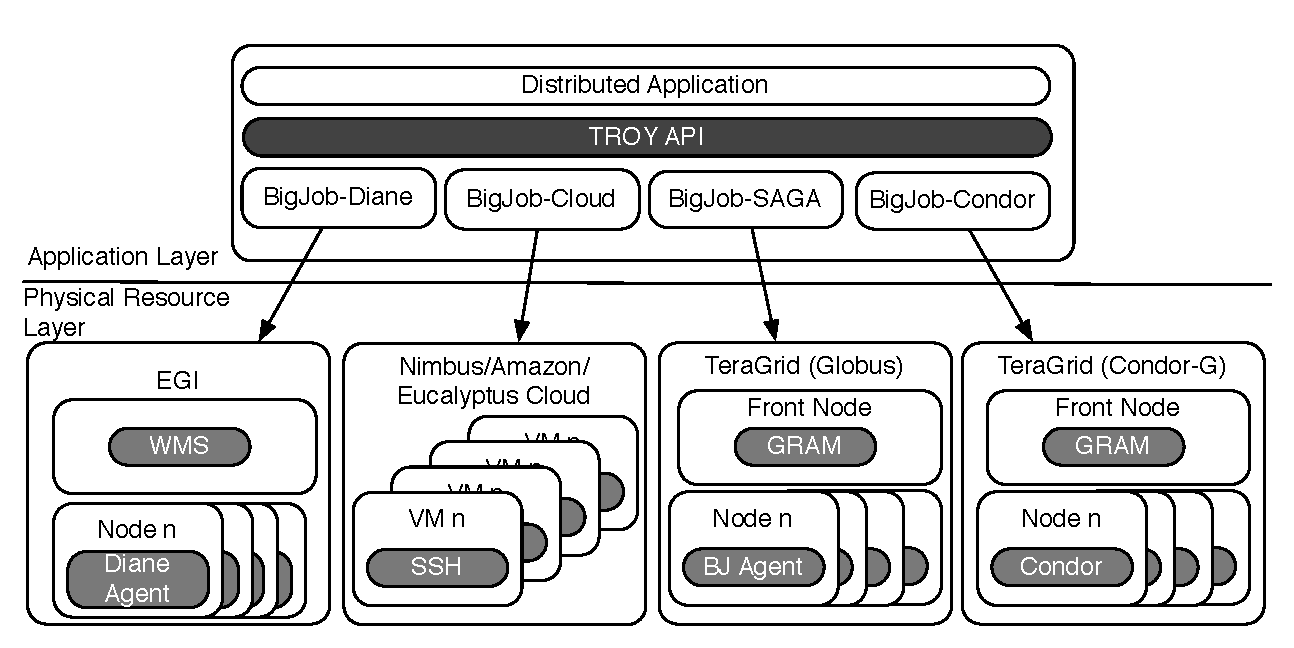
\includegraphics[width=0.48\textwidth]{figures/distributed_pilot_job.pdf}
    \caption{\textbf{Pilot-API and PJ frameworks:} The Pilot-API provides 
      a unified interface to utilize the native Pilot-Job capabilities of
      different infrastructures, e.\,g.\ BigJob for XSEDE/Cloud
      resources, DIANE for EGI and Condor for OSG resources.
%       It also enables the concurrent usage of these infrastructures.
	\upp\upp\upp}
    \label{fig:figures_distributed_pilot_job}
\end{figure}

% \begin{figure}[t]
% 	\upp
% 	\centering
% 		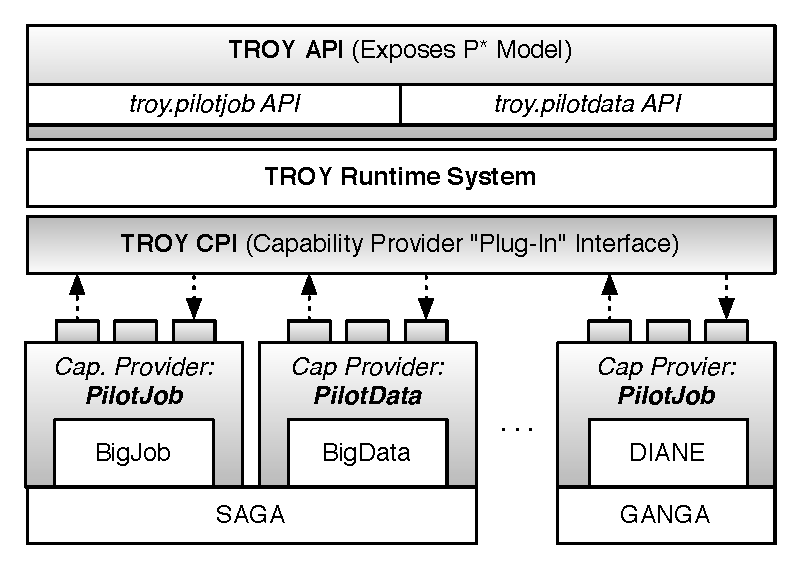
\includegraphics[width=0.45\textwidth]{figures/TROY_arch.pdf}
%                 \caption{\textbf{TROY -- An API and Runtime System for
%                     the P* Model:} TROY provides an API for managing
%                   PJs and PDs. BigJob and BigData are realizations of
%                   the actual PJ and PD functionality. BJ and BD rely
%                   on SAGA for implementation of the PJ/PD.
% 	\label{fig:figures_pstar_troy}
% 	\upp\upp
% \end{figure}

Figure~\ref{fig:figures_troy_flow} shows the interactions between the
P* elements. The Pilot-API decouples workload management and resource
scheduling by exposing two separate services: The
\texttt{PilotService} (PS) and \texttt{ComputeUnitService} (CUS). The
PS serves as a factory for instantiating pilots. Also, the PS can be
used to query the PJS for currently active pilots.  A
\texttt{Pilot} object is returned as result of the
\texttt{create\_pilot()} method of the PS (step 1).

As in SAGA, the instantiation of \texttt{Pilot} object is done by
using a \texttt{PilotDescription}. The description can be reused
and has no state, while the \texttt{Pilot} instance has state and
is a reference for further usage.

\lstset{
language=Python,
frame=single,
captionpos=b,
stringstyle=\ttfamily,
basicstyle=\scriptsize\ttfamily
}

\noindent\begin{minipage}{0.47 \textwidth}
\begin{lstlisting}[caption={\textbf{Pilot Creation:} Instantiation of a Pilot Service using a Pilot Description.}, label={lst:ps_creation}]
ps = PilotService()
p_desc = PilotDescription()
p_desc.total_core_count = 8
pj = ps.create_pilot('gram://queenbee', 
                          p_desc, 'bigjob')
\end{lstlisting}
\end{minipage}

The \texttt{Pilot} object represents a pilot instance and allows the 
application to interact with a pilot, e.\,g.\ to query its state or to cancel 
it. The process of Pilot creation is depicted in step 1-3 of 
figure~\ref{fig:figures_troy_flow} and in listing~\ref{lst:ps_creation}.

Listing~\ref{lst:cus_creation} shows the creation of a
\texttt{ComputeUnitService}.
Having instantiated a \texttt{ComputeUnitService} object, PS objects can be
added and removed at any time. This enables applications to respond to dynamic
resource requirements at runtime, i.\,e.\ if peak demands arise an application
can request additional resources; if resources are not required anymore, they
can be released.

\noindent\begin{minipage}{0.47 \textwidth}
\begin{lstlisting}[caption={\textbf{ComputeUnitService Creation:} Instantiation
of a \texttt{ComputeUnitService} using a reference to the
\texttt{PilotService}.}, label={lst:cus_creation}]
cus = ComputeUnitService()
cus.add(pjs)
\end{lstlisting}
\end{minipage}

\noindent\begin{minipage}{0.47 \textwidth}
\begin{lstlisting}[caption={\textbf{ComputeUnit Submission:} Instantiation and 
	submission of a \texttt{ComputeUnitDescription}.}, label={lst:submission}] 
cud = ComputeUnitDescription()
cud.executable = '/bin/bfast'
cud.arguments = ['match', '-t4', '/data/file1']
cud.total_core_count = 4
cu = cus.submit(cud)
\end{lstlisting}
\end{minipage}

% \lstset{
% caption={\textbf{WorkUnit Submission:} Instantiation and Submission of a \texttt{WorkUnitDescription}.\label{lst:submission}}
% }

The \texttt{ComputeUnitService} is responsible for managing the execution of \cus.
Regardless of the state of the PS, applications can submit \cus to a
\texttt{ComputeUnitService} at anytime (listing~\ref{lst:submission} and step 4 in
figure~\ref{fig:figures_troy_flow}). Once the \texttt{ComputeUnitService} becomes
responsible for a \cu, the \cu  transitions to an SU. SUs are internally processed
(they e.\,g.\ can be aggregated) and are then forwarded to the
\texttt{Scheduler} (step 5), which selects an appropriate pilot. Having chosen
an appropriate resource, the SU is dispatched using the respective adaptor (step
6 and 7). The PJ framework is responsible for the actual execution of the SU on
a resource
Note that multiple levels of (hierarchical) scheduling can be
present, commonly a SU is scheduled inside a PJ framework and the model allows
it to be present in multiple layers.



% In figure~\ref{fig:figures_troy_flow} the flow of a simple execution scenario is
% displayed. The Pilot Job Service and the Work Unit Service are already
% instantiated. The application requests the Pilot Job Service to create a new
% pilot-job (step 1), the Pilot Job Service will pass the request on to the
% relevant adaptor (step 2), which will eventually launch the pilot-job on a
% resource using a pilot-job framework (step 3). At this stage there might be a
% pilot-job already available, or the request can still reside in a queue
% somewhere. Regardless of the state of the pilot-job, the application can submit
% a work unit to the Work Unit Service (step 4). The Work Unit Service remains
% responsible for keeping track of the Work Unit during its lifetime. Based on the
% heuristics or policies the WUS decides on a potential aggregation of SUs. The SU 
% is then forwarded to the Scheduler (step 5). The Scheduler will schedule SUs to 
% an appropriate adaptor that represents a capable resource (step 6). Finally, the
% adaptor will submit the SU to the PJ framework which will
% take care of the actual execution on a resource. Note that multiple levels of 
% (hierarchical) scheduling can be present. Inside
% TROY there is already scheduling taking place inside the Work Unit Service. 
% Additionally, the underlying PJ framework can conduct its own scheduling.


Each \texttt{ComputeUnit} and the \texttt{Pilot} object is associated with a
state. The state model is based on the SAGA job state
model~\cite{ogf-gfd-90}.
\note{OW says: Why? IMHO the GFD.90 state model has some serious flaws, like
the absence of a 'Waiting' state.} 
Applications can query the state using the \texttt{get\_state()} method or they
can subscribe to state update notifications.

Semantics:
An application can have any number of PilotServices or ComputeUnit Services.
Multiple PilotServices can be associated to a ComputeUnitService, and a
PilotService can be associated to multiple ComputeUnitServices. A
ComputeUnitService can manage multiple ComputeUnits, but a ComputeUnit can only
be managed by one ComputeUnitService. So can a PilotService manage
multiple Pilots, but can a Pilot only be managed by one PilotService.

The Pilot-API supports different usage modes i) it provides a unified API to
various PJ frameworks (e.\,g.\ BigJob, DIANE and Condor-G), and ii) it enables
the concurrent usage of multiple PJ implementations. 

\begin{figure}[t]
	\centering
		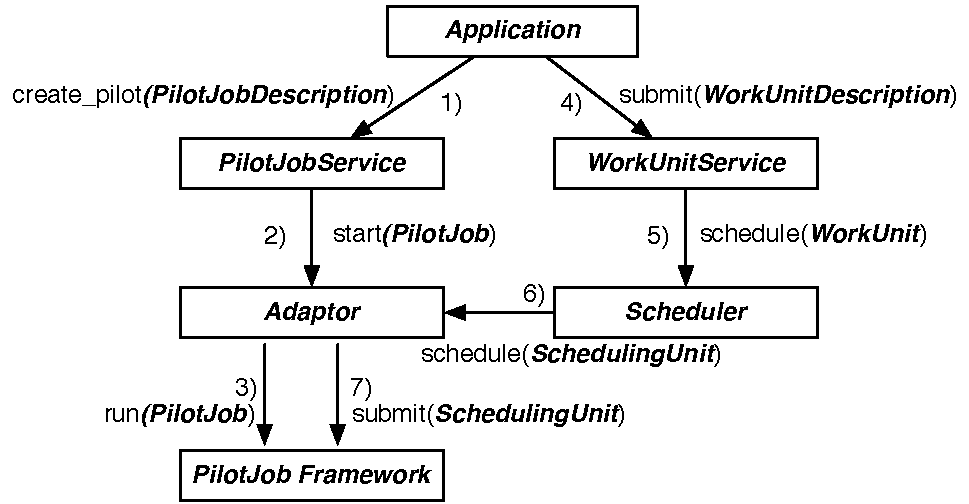
\includegraphics[width=0.47\textwidth]{figures/troy_flow.pdf}
	\caption{\textbf{Control Flow Pilot-API and PJ Frameworks:} The functionality    of pilot-jobs are exposed 
	using two primary classes: The \texttt{PilotService} for the management 
	of pilots, and the \texttt{ComputeUnitService} for the management of \cus.
    \alnote{figure needs attention.}
	}
	\label{fig:figures_troy_flow}
\end{figure}

\begin{table}[t]
	\centering
\begin{tabular}{|l|l|}
\hline
\textbf{Pilot} &PJ framework\\
\hline
\textbf{\cu } &\cu \\
\hline
\textbf{SU} &SU\\
\hline
\textbf{Pilot-Manager} & PilotService/ComputeUnitService\\
\hline
\end{tabular}
\caption{Mapping of P* and the Pilot-API\upp\upp}\label{table:pstar_elements}
\end{table}

The Pilot-API classes and interactions are designed to reflect the P*
elements and characteristics.
Table~\ref{table:pstar_elements} summarizes the mapping of P* elements and the
Pilot-API. As defined by P*, a \cu represents a primary self-containing piece
of work that is submitted through the Pilot-API. 
At the API boundary a \cu transitions to a SU, which functions as internal unit
of scheduling.
The API follows object-oriented design principles and exposes the primary
functionality of the Pilot-Manager using two classes: the
\texttt{PilotService} for the management of pilots and the
\texttt{ComputeUnitService} for the management of \cus. 
Further, the framework utilizes a set of internal classes for implementing
different P* characteristics, e.\,g.\ the \texttt{Scheduler} for scheduling and
the adaptors implementations for providing the actual PJ capabilities.


\section{Experiments and Results\upp\upp}
\label{sec:exp_res}
% In this section we discuss the TROY API. Further, (i) we show that
% the TROY API can be used to marshal DIANE stand-alone as well as
% (ii) that the TROY API can be used stand alone with both BigJob and
% DIANE concurrently.

\jhanote{MS: The experiment section needs tighter and more focussed
  writing in general}

In this section we analyze the performance and scalability of different PJ
frameworks. The experiments are conducted on different production (XSEDE, EGI,
OSG) and research infrastructures (FutureGrid). In
section~\ref{sec:pj_performance} we investigate the performance and scalability
of BigJob and DIANE executing a simple shell command. In
section~\ref{sec:fg-xsede-osg-egi} we show that the execution of {\it real
application workloads} -- in this case a genome sequencing application --
on production infrastructure is a strength of our approach and capabilities.
Further, we demonstrate PJ framework interoperability by using multiple PJ
frameworks concurrently on multiple production infrastructures using the
Pilot-API.

It should be noted that our experiments do not try to identify the ``best'' or
``fastest'' PJ framework, as this is dependent on different factors, e.\,g.\
particularly the used infrastructure. As established early, the investigated PJ
frameworks can be mapped to the P* model and the Pilot-API, which enables the
collective usages of these frameworks.

\jhanote{Need a simple description of experiment   configuration}.
\alnote{Is it ok to just describe the configuration on high-level in the 
introduction and do this in detail in the sub-sections?}

% \alnote{this paragraph is redundant to B and C? Alternative we can move
% stuff from there to here.}
% For purposes of validation, demonstration and performance
% measurements, we use the Pilot-API to marshall different PJ
% frameworks...  The experiments are conducted on different
% production (XSEDE, EGI, OSG) and research infrastructures
% (FutureGrid).

\jhanote{Need to provide details of the application} 
\alnote{Is it ok to do this in subsection B and C?}

%(with SAGA/PBS and SAGA/Condor) and DIANE in a genome sequencing
%application scenario.



% \amnote{Someone please check the above statement for sanity!}
% \alnote{What's a concertation?}  \amnote{wiktionary says: "A form of
%   dialogue and co-decision, implying the mutual exchange of
%   information, open discussion and knowledge sharing, and the
%   signature of operational agreements between public administrations
%   and/or with representatives of the private sector."  Basically
%   means in our context 'in a coordinated way, in
%   combination'.}\jhanote{Would `` collectively'' be a better
%   description?}

\subsection{Understanding Coordination in PJ Frameworks\upp\upp}
\label{sec:pj_performance}
\alnote{Explain why /bin/date!}

Each PJ implementation is associated with various degrees of freedom,
in particular in the design of the communication \& coordination
(c\&c) sub-system.  The primary barrier for performance and
scalability is not the \cu  submission, but the internal coordination of
the elements of a P* implementation. There are many factors that
influence the overall performance, e.\,g.\ the degree of distribution
(local (LAN) vs. remote (WAN)), the communication pattern (1:n versus
n:n) and the communication frequency. In the following we investigate
the impact of different c\&c related factors on the overall
performance and scalability of the system.

The original design of BigJob is based on a shared, centralized data
space, the SAGA Advert Service~\cite{saga_advert}, which is
essentially a PostgreSQL database. The communication between all
components is done via this data space; this concept is also known as
tuple space~\cite{Gelernter:1985:GCL:2363.2433}.  The data space
decouples BJ-Manager and BJ-Agent very well and allows both entities
to operate at their own pace optimizing the overall throughput.
Depending on the setup this data space can be deployed locally,
i.\,e.\ on the same resource, or remotely, e.\,g.\ during a
distributed run. A particular issue during distributed runs is the
latency between the application and the Advert Service. Another
challenge is that this design introduces a potential
single-point-of-failure and scalability bottleneck if the centralized
data space is not carefully designed and operated.


BigJob also provides two alternative c\&c sub-systems:
Redis~\cite{redis} and ZeroMQ~\cite{zmq}. Redis is a lightweight
key/value store, which can be deployed in a distributed, fault
tolerant way. Redis is used in a similar way as the Advert database,
i.\,e.\ all communication between BJ-Agent and manager is channeled
through it. Redis can be deployed locally and remotely.  The ZeroMQ
c\&c sub-system in contrast utilizes a client-server architecture,
which is similar to the CORBA-based~\cite{OMG-CORBA303:2004}
communication system of DIANE. In this architecture, the PM maintains
the overall state. Clients connect to the PM to request new SUs or to
report state updates. An advantage of this architecture is that it
does not require a separate infrastructure for deployment of the
Advert Service or the Redis database. While the BJ-Manager can be
deployed remotely from the BJ-Agent, in most cases this will not be
the case, i.\,e.\ the communication between BJ-Manager and BJ-Agent is
mostly local communication. Both the data space and client-server c\&c
sub-system can be combined with a publish/subscribe mechanisms,
i.\,e.\ instead of polling an agent or client can receive
notifications when a new SU arrives. 

We evaluate different BJ configurations and compare and contrast them with
DIANE. For this purpose, we conducted several experiments on
FutureGrid~\cite{fg}. To evaluate the overall performance and throughput, we
execute a different number of \cus on Alamo and Sierra utilizing up to 128 cores
concurrently. Since the purpose of the experiment is to evaluate the performance
and scalability, we execute a set of very short-running \cus concurrently. Each
\cu runs a single \texttt{/bin/date} command. This enables us to focus on the
overhead induced by the PJ framework and the c\&c subsystem. Each experiment is
repeated at least 10 times.

% \jhanote{Need to motivate testing of c\&c sub-system better: There are
%   many barriers to interoperability and performance. primary barrier to
%   performance is not \cu  submission or SU scheduling to PM, but the
%   fundamental limitation of scalability of coordination -- with
%   increasing number of \cu /SU.  Establish tradeoff between distributed
%   vs local coordination. e.g., It is easy to get consistency but has
%   overhead.  Easy to get performance but difficult to get
%   consistency. Thus we opt for centralized / persistent point. But how
%   does this single point-of-coordination behave with increasing number
%   of connections? } \alnote{hopefully addressed most points in paragraph above}

% \begin{figure*}[htbp]
% 	\centering		
% 	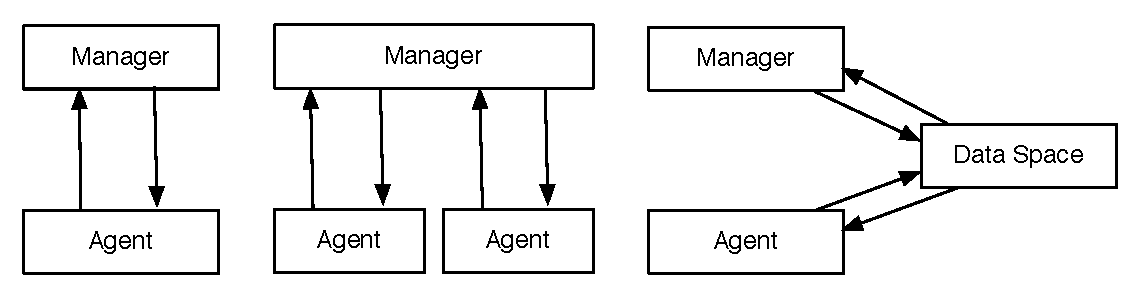
\includegraphics[width=0.8\textwidth]{figures/coordination-schemes.pdf}
% 	\caption{\textbf{Coordination \& Communication:} The primarily used 
% 	coordination pattern is the utilization of a request/response server 
% 	(left, middle). In the data-space model (right) all application components 
% 	are connect to a central data-space. This architecture decouples manager 
% 	and agent allowing both to operate on its own pace.}
% 	\label{fig:figures_coordination-schemes}
% \end{figure*}

% Figure~\ref{fig:figures_coordination-schemes} illustrates different
% coordination schemes. 

% Most pilot-jobs utilize the master-worker \jhanote{M-W for what?}
% pattern commonly implemented on basis of a simple request/response
% architecture, i.\,e.\ the \jwave{agent} sends a request for work
% packages to the master, which replies with a \cu . 

% \jhanote{Are we talking specific implementation, i.e., TROY? If so we
%   should not say ``A'' manager but ``The Pilot-Manager''? Also the previous
% sentence should not talk about most pilot-jobs, if we've already started
% talking about TROY!!} \alnote{hopefully fixed.} 

% A manager
% can manage a single agent (e.\,g.\ BigJob) or multiple agents
% (e.\,g.\ DIANE). 


\begin{figure}[htbp] \centering
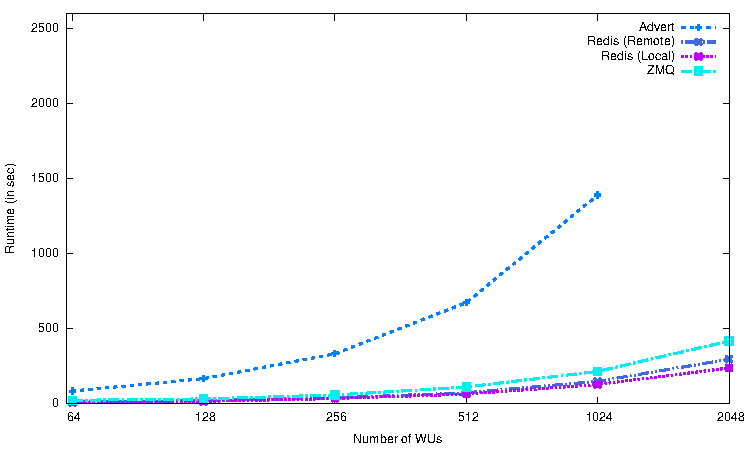
\includegraphics[width=0.49\textwidth]{perf/bigjob-varying-wus-alamo.pdf}
\caption{\textbf{BigJob and DIANE Performance (1):} The 
time-to-completion for $n$ \cus scales linearly
in most cases, i.\,e.\ the coordination overhead imposed by the BJ is 
minimal.\upp\upp}
\label{fig:perf_bigjob-varying-wus} \end{figure}

Figure~\ref{fig:perf_bigjob-varying-wus} illustrate the performance and
scalability of the different BigJob configurations and DIANE with respect to the
number of \cus. Clearly, the used c\&c sub-system has a great impact on the
overall performance. The Redis backend shows the best performance for small \cu 
counts. The difference between local and remote coordination is moderate (about
20\,\%). While ZeroMQ is very fast and lightweight, it requires a careful
implementation in particular concerning synchronization and throughput
optimization. The overall performance is slightly worse than for Redis. The
Advert Service currently has some limitations which will be discussed later.
DIANE shows a higher startup overhead, which is particularly observable for
smaller \cu  numbers. However, the runtime increases only slightly (about 10\,sec)
when going from 64 to 2048 \cus. A reason for this behavior is that DIANE
aggregates SUs: for 2048 \cus only a single task description is created, which
the framework then efficiently distribute to its worker agents. BigJob in
contrast maintains for each \cu  a separate description. 
% At the investigated
% scales, the single manager does not represent a bottleneck with respect to the
% processable \cu  numbers. Further, the TROY manager introduces another 
% hierarchy-level which can further
% enhance the overall scalability.

Figure~\ref{fig:perf_bigjob-varying-cores} illustrates the performance
scalability with respect to the number of cores. In particular, the Redis
(Local) configuration show an almost linear scalability up to 128 cores. The
Redis remote setup again imposed some overhead (about 14\,\%). ZeroMQ performs
very well with lower core counts; with larger core counts the runtimes increase
indicating a potential scalability bottleneck. DIANE shows in particular for
lower core counts a longer runtime again due to the higher startup overhead.
With higher core counts DIANE behaves similar to BigJob ZeroMQ showing a greater
increase of the overall runtime. This increase can likely be attributed to
the single central manager in the client-server architecture. As in the last
experiment, the Advert c\&c sub-system showed a significantly lower performance.

\begin{figure}[htbp] \centering
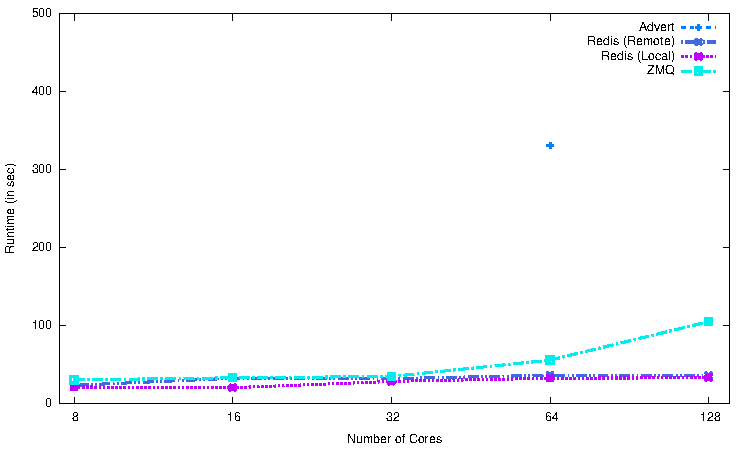
\includegraphics[width=0.49\textwidth]{perf/bigjob-varying-cores-alamo.pdf}
\caption{\textbf{BigJob and DIANE Performance (2):}  The
runtime of a constant workload of 4 \cus 
increases only slightly up to 128 cores. In particular, the Redis backend shows
an almost linear scalability achieving a throughput of up to 4 \cus/sec. }
\label{fig:perf_bigjob-varying-cores} 
\upp\upp
\end{figure}

The BigJob Advert implementation currently shows some performance
limitations mainly caused by the prototypical nature of the Advert
Service implementation.  Further, it must be noted that the Advert
Service was deployed remotely (mainly due to deployment
constraints). However, even considering this aspect the discrepancy
between Advert Service and Redis (Remote), which has been deployed on
the same remote network, is significant. A reason for the worse
performance is the used remote access protocol. The Advert Service is
based on PostgreSQL; in the current architecture the client, i.\,e.\
the BJ-Manager and agent access the PostgreSQL database via the SOCI
backend library. While this architecture provides a very flexible
remote access to the database, running database access protocol over a
WAN connection is not optimal. % \jhanote{It is not clear why REDIS and
%   ZeroMQ are not susceptible to access over WAN
%   delays/latency?}\alnote{included a comparison note to Redis
%   Remote. We can't compare it to ZMQ since we use only local
%   communication in this case}
Transactions e.\,g.\ are very latency sensitive and require several
roundtrips.  Further, the API is based on a hierarchical namespace,
which does not naturally map well to relational databases. In
particular deeply nested namespaces exhibit an insufficient query and
update performance. In contrast, both in the Redis and ZeroMQ
scenario, data is stored in memory, which also explains to significant
performance gains.

\upp

\subsection{Characterizing PJ Frameworks on Production Infrastructure\upp\upp}
\label{sec:fg-xsede-osg-egi}

\subsubsection*{Production Infrastructure} To validate the abstractions
developed, we conducted a series of experiments on various production
infrastructure. We execute BFAST~\cite{bfast2009} -- a genome sequencing
application -- using different PJ frameworks, i.\,e.\ BigJob, DIANE and Condor,
and infrastructures, i.\,e.\ XSEDE, FutureGrid, EGI and OSG. On XSEDE, we
utilize Kraken, a 1.17 PF machine with a total of 9,408 nodes and 112,896 cores;
on FutureGrid we utilize India, a 108 node cluster with 864 cores.

\note{Add OSG, EGI details ...}
 
\jhanote{Experimental Configuration = Infrastructure used, specific
  machine (on XSEDE and FG) and resources configuration + PJ Framework
  employed.}


\jhanote{I would even introduce a sub-subsection on production
  infrastructure used. That would enable us to keep Pilot-API/BigJob
  specific details separate from infrastructure details. E.g., say
  what is XSEDE? Say what is OSG? Thoughts?}
\alnote{good idea. started to restructure section}


%\note{OW says: That would be the case if we use Condor-G. The machines
%is belhaven-1.renci.org - a Globus/PBS cluster that accepts Condor jobs.\\
%So the OSG is a peculiar beast. My current understanding is, that it consits 
%of a bunch of HPC clusters with a Globus frontend. OSG uses an automated 
%Glide-in WMS service that starts glide-ins via Condor-G on these clusters.
%The glide-ins are aggregated and presented to the OSG (HTC) user as a 
%standard condor pool for HTC jobs. While using OSG through condor seems 
%to be a popular mode of operation, it is possible to access any of the 
%OSG-member clusters via Condor-G and through Globus directly. As far as I
%understand, this is the preferred mode for running HPC (multi-core) 
%applications.\\
%This raises two important questions: does it make sense it all to use
%BigJob with the OSG condor pool? We would end up with one BJ agent per
%condor job which represents one core, which would just add a lot of overhead and
%no benefits. Using OSG via Condor-G or even Globus would allow us to
%take advantage of larger reservations, e.g. one BJ agent that manages
%128 cores.\\
%While it would make sense for TROY to implement a native Condor 'backend'
%that doesn't use another layer of 'agents' and master/worker advert 
%mechanisms, I don't think that this makes sense for BigJob. Depending on 
%what we want to show, I propose that we use BigJob with Globus (we now that 
%it works) on OSG. While this doesn't show pilot job interoperabiltiy
%(which his hard to achieve without TROY anyways), it still shows cross-grid
%interoperability.}


% To manage the genome sequencing workflow we use
% theDARE~\cite{dare-tg11-gateways} framework that has been built on
% top of TROY.

\subsubsection*{Experimental Configuration}

The investigated workload comprises of 128 \cus. Each \cu executes a BFAST
matching process, which is used to find potential sequence alignments. The
scenario requires about 7\,GB input data: 1.7\,GB for the reference genome and
index files and 5.4 GB read files (32 files a 1.68\,GB). We run the experiment
on four different setups: (i) BigJob/XSEDE only, (ii) BigJob/FutureGrid, (iii)
BigJob/OSG only, (iv) DIANE/EGI only. 


To achieve interoperability, we developed a Pilot-API interface to all three PJ
frameworks, i.\,e.\ BigJob, DIANE and Condor. The Pilot-API provides a unified
way to access the different native PJ capabilities. For the experiments we rely
both on the native PJ APIs, in particular the BJ API, and the 
Pilot-API.\jhanote{The
  last sentence is confusing. Second last sentence needs to be
  explained better and the two need to be reconciled}
The following PJ setup was used: BigJob is used with the SAGA-Torque adaptor to
access Kraken on XSEDE~\cite{xsede} and with the PBS/SSH plugin to access the
India machine on FutureGrid~\cite{fg}. For OSG we utilize a BJ implementation on
top of the SAGA/Condor adaptor.\note{Refine: GlideWMS, ...}
resources~\cite{1742-6596-78-1-012057}. Further, we utilize DIANE on EGI.
\msnote{more on EGI later ...} On the XSEDE, Kraken is used with up to 512 cores
concurrently.


Each BFAST \cu requires 1 core; In each case 128 \cus are defined and submitted
to the Compute Unit Service. Depending on the resource, a different number of
cores can be reserved to each BFAST \cu, e.\,g.\ on Kraken 4 cores are reserved
for each \cu. Each \cu is associated with a set of input files which is
pre-staged in case (i) and (ii). For the HTC infrastructures: EGI and OSG (case
(iii) and (iv)), these file are transferred before running each \cu. \alnote{Are
the files staged once for each \cu?} Having submitted the 128\,\cus, the
benchmark application can monitor the state using the Compute Unit Service of
the Pilot-API.

\begin{figure}[t]
	\centering
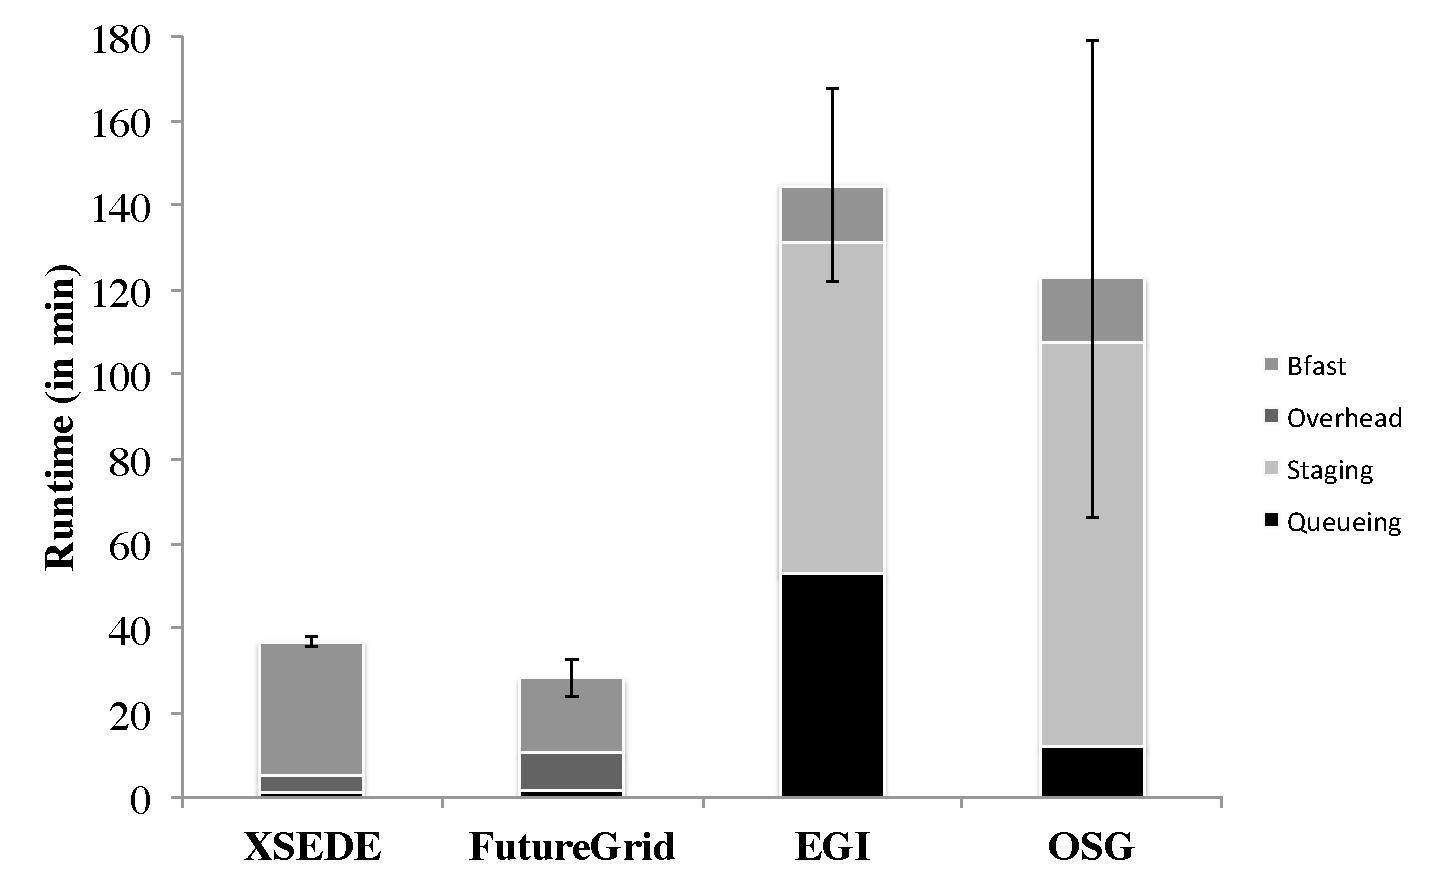
\includegraphics[width=0.45\textwidth]{perf/interop/128-bfast-egi-fg-xsede-osg.pdf}
\caption{\textbf{PJ Framework Performance on XSEDE, FutureGrid, EGI and 
OSG:} Running 128 BFAST match tasks on 128 cores. Each experiment is
          repeated at least 3 times. The runtime on EGI and OSG is higher
          mainly caused by the longer queuing and staging time. Additionally, 
		  both 
		  infrastructure require the staging of all input files. 
		\up\up}

	\label{fig:perf_perf-bfast-bj}
\end{figure}

Figure~\ref{fig:perf_perf-bfast-bj} shows the results of the experiments. In
addition to the runtime we measured the queuing time, i.\,e.\ the time 
required until a \cu changes its state to running, the time necessary to 
transfer the input files, and the actual runtime of the BFAST \cu. The queue 
time include both pilot-external, i.\,e.\ waiting times at the RM system, as 
well as pilot-internal waiting times.

% BFAST PERFORMANcE
Generally, the performance of BFAST is
heavily dependent on the available IO. Both the index and read files (6\,GB in
this scenario) need to be loaded into memory. Both resources deploy a shared
filesystem: Lustre in case of Kraken and NFS in the case of India. Since the
file system is a shared filesystem, the performance of BFAST particularly 
degrades on larger machines, such as Kraken, where many jobs access the same 
resource. Thus, the runtime on Kraken is about 30\,\% slower than on India.
Both on EGI and OSG, the  BFAST match \cu performs the best: on OSG is about two 
times faster than on Kraken. This can mainly be attributed to the usage of local 
storage on these HTC infrastructures.

% Queuing Time
Another important factor is the queueing time. In scenario (i) and (ii), the
queueing times at the time of the experiments have been very low. The main part
of the queuing time is attributed to the BJ internal queue, i.\,e.\ for queuing
the sub-jobs to a BJ agent. In the EGI/DIANE case (iii), the queuing time is
mainly attributed to the launch of the 128 worker agents. Each of these agents
needs to be submitted and started via the WMS. On each node a DIANE worker agent
must be downloaded, installed and started separately. In total, each \cu was
required to queue about 50\, minutes in comparison to 9\,minutes queuing time
for BJ on India (FG). Thus, even if the file staging time is not considered, the
scenario executes about 2.3 times slower on EGI (DIANE) than on FutureGrid (FG).
The unpredictable queuing time also contributes to the higher deviation in the
measured runtimes. On OSG the queuing time is in average 12 minutes, which is
comparable the queuing time on XSEDE.

% File Staging
In the scenarios (i) and (ii) no file staging is used. On EGI and OSG resources,
however, no shared filesystem is available; thus, files needs to be transferred
to the execution machine. For each \cu, the reference genome, the index files
and one read file need to be staged (3.38\,GB). More than 50\,\% of the runtime
is required for staging the input files. Thus, the runtime on these two
infrastructures is about 4-5 times longer than on Kraken and India. If file
staging is not considered, OSG shows the best performance of all scenarios
(i)-(iv).



% Despite the fact that BigJob has been also installed
% with each run, it shows a significant lower startup time of 73\,sec, i.\,e.\
% about 50\,sec less than DIANE. Additionally, we also observed a runtime
% overhead of about 25\,sec for the DIANE scenario. This overhead is likely
% caused by the additional agents required. While BigJob utilizes one BJ-Agent
% on the resource, DIANE currently requires the spawning of one worker agent per
% \cu that must be executed in parallel. While the Pilot-API marshals these
% differences, i.\,e.\ while the API remains the same for both PJ frameworks, a
% light performance overhead remains observable.


% This
% can mainly be attributed to the better performance of the OSG resource, which is
% particularly visible in the BFAST runtimes, which are on average 40\,\% shorter
% than on LONI. Further, due to the lack of SAGA on OSG, BJ is deployed with the
% Redis c\&c sub-system, which shows a significantly better performance than the
% Advert Service (see section~\ref{sec:pj_performance}).

% \jhanote{What are we trying to say here?  Is it that although the API
%   is similar, semantics of implementation and execution remain
%   different, and that TROY backend handles them?}\alnote{well said}


% This part also sounds too engine-like
% Dynamic
% applications can utilize the elasticity of the TROY resource pool
% e.\,g.\ to improve the time-to-completion and/or to scale the accuracy
% of their computations.

\subsection{Understanding PJ Framework Interoperability\upp\upp}
\label{sec:experiment-interop}

We define two kinds of interoperability: (i) SAGA-based
interoperability, i.\,e.\ the usage of BJ in conjunction with
different SAGA adaptors and infrastructures and (ii) PJ framework
interoperability, i.\,e.\ the usage of different PJ frameworks via the
Pilot-API. For scenario (i) we run BigJob concurrently on FutureGrid
and XSEDE and for scenario (ii) we concurrently run BigJob and DIANE
on FutureGrid and EGI.

\begin{figure}[htbp]
	\centering
	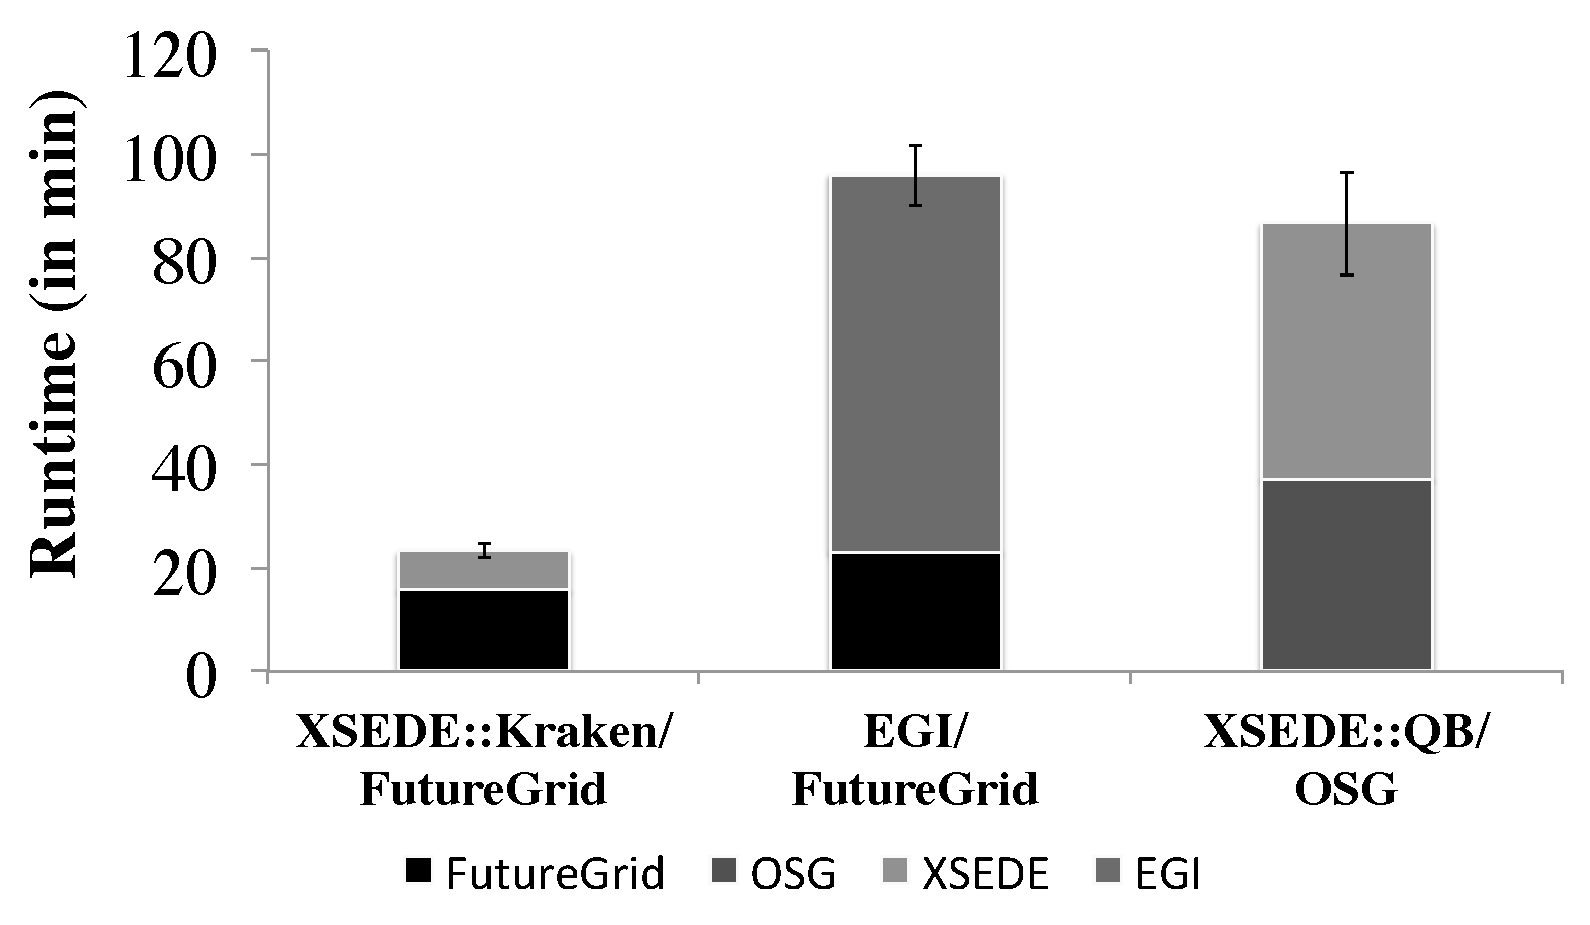
\includegraphics[width=0.45\textwidth]{perf/interop/128-bfast-interop.pdf}
	\caption{PJ Framework Interoperability}
	\label{fig:perf_interop_128-bfast-interop}
\end{figure}


Figure~\ref{fig:perf_interop_128-bfast-interop} shows the results of the
interoperability tests. In both scenarios, one \pilot is submitted to each
infrastructure. In scenario (i), one pilot is submitted to Kraken and one to
India. Needless to say, the overall runtime is determined by the slower
resources. Consistent with previous results the \pilot on India finished before
the \pilot on Kraken.


\jhanote{should this scenario number be
  different?} \alnote{sorry, just moved this paragraph down from B}
Finally, scenario (ii) demonstrates that two PJ frameworks can be utilized
concurrently using the Pilot-API. The performance in this scenario is
slightly better than in the DIANE only case, mainly due to the fact
that only four DIANE worker agents need to be started. Also, only half
of the \cus are executed on a DIANE node and thus, show a longer
runtime. While there are some limitations in the current DIANE
implementation, the aim of this experiment is to emphasizes the
possibilities that the Pilot-API provides to dynamic applications. The
Pilot-API enables applications to utilize a dynamic resource pool
consisting of resources of different infrastructures, e.\,g.\ EGI and
TG/XD resources, at large-scales hitherto unattainable.


Motivate:

- inefficient file staging -- for Condor and DIANE all input files are staged 
separately for each sub-job



\section{P* as a Model for Pilot-Data\upp\upp}
\label{sec:pilot-data}
\alnote{remove emphasis on dynamic execution} \jhanote{Motivation for
  P* model for data: (i) Distributed data placement not done
  effectively or scalably; (ii) unable to handle dynamic
  (late-binding) issues or multi-stage dependencies, (iii) further
  optimizations}

Many scientific applications have immense data requirements, which are projected
to increase dramatically in the near future~\cite{hey2009}. The small genome
sequencing application scenario presented above e.\,g.\ operates on a input data
set of $>7$\,GB. While Pilot-Jobs efficiently support late-binding of
\computeunits and resources, the management of data in distributed systems
remains a challenge due to various reasons: (i) The placement of data is often
decoupled from the placement of compute units and pilots, i.\,e.\ the
application must often manually stage in and out its data using simple scripts.
(ii) Heterogeneity, e.\,g.\ with respect to storage, filesystem types and paths,
often prohibits or at least complicates late binding decisions. (iii)
Higher-level abstraction that allow applications to specify their data
dependencies on an abstract, logical level (rather than on file basis) are not
available. (iv) Due to lack of a common treatment for
compute and data, optimizations of data/compute placements are often not
possible. For example, in scenario (iii) and (iv) presented in
section~\ref{sec:fg-xsede-osg-egi}, even though the 50\,\% of the input data set
is shared for all \cus, the complete data is staged for each \cu.

In addition, applications must cope with various other challenging, data-related 
issues, e.\,g.\ varying data sources (such as sensors and/or other
application components), fluctuating data rates, transfer failures,
optimizations for different queries, data-/compute co-location etc. While these 
issues can be in principal handled in a application-specific way, the usage of
higher-level abstractions, such as a common \pilot-based abstraction for compute 
and data is preferable.

% Thus, having
% defined the P* model, we explore its extension to data.

This will motivate an analogous abstraction that we call
\emph{\pilotdata (PD)}. \jwave{PD provides late-binding capabilities
  for data by separating the allocation of physical storage and
  application-level data units.}  Further, it provides an abstraction
for expressing and managing relationships between data units and/or
work units. These relationships are referred to as \emph{affinities}.

% \jhanote{difficult to use affinity without defining it..}
% \alnote{tried to describe affinities a little bit better}

%\alnote{Extension vs. Application vs. Translation}
\subsubsection*{P* Model Elements for Data}

% A Pilot-Data Framework facilitates the late-binding between data units
% and physical storage resources, the so called pilot-stores.

The elements defined by P* (in section~\ref{sec:p_star_elements}) can
be extended by the following elements:

%\alnote{What is the role of SU in Data?}
\begin{compactenum}[A.]

\item \textbf{\pilot (Pilot-Data):} A \pilotdata (\pd) functions as a 
	placeholder object that reserves the space
	for data units. PD facilitates the late-binding of data and resource and is
	equivalent to the \pilot in the compute model.

\item \textbf{Data Unit (DU):} DU is the base unit of data assigned by
  the application,  e.\,g.\ a data file or chunk. Multiple DUs can be aggregated 
   within a Data Unit Set.

% \item \textbf{Pilot-Data (PD):} PD allows the logical grouping of DUs
%   and the expression of data-data affinities. This collection of files
%   can be associated with an extensible set of properties. One of these
%   properties is affinity. 

\item \textbf{Scheduling Unit (SU):} is an internal unit of scheduling (as in 
the compute model). The Pilot framework can can aggregate or split DUs into one 
or more SUs.

\item The \textbf{Pilot-Manager (PM)} is the same as in the compute model and
implements the different characteristics of the P* model. It is responsible for
managing \dus and \sus. Data is submitted to the framework via the PM. The PM
which is responsible for mapping \dus to \sus and for conducting decision 
regarding resource assignments. \sus are placed on physical resources via the \pilot.
	
\end{compactenum}
 
Note, each element can be mapped to an element in the P* Model by
symmetry, e.\,g., a DU correspond to a \cu  in the original P* Model; 
a PD is a placeholder reserving a certain amount of storage on a physical 
resource and corresponds to the \pilot in the P* Model.

% \jhanote{PJ Model is confusing. Either it is P Model or PJ
%   Framework} \alnote{ok}

% A particular critical requirement for data-intensive application, is
% the management of affinity between DUs and also between \cus and
% DUs. Thus, Pilot-Data introduces the PD container object for
% expressing relationships between DUs. A PD corresponds to an SU in
% the \jwave{PJ model}, i.\,e.\ it is used as scheduling unit for
% internal optimizations, e.\,g.\ the grouping of DUs. Having
% instantiated a PD, it can be assigned to a PS via the PD manager. A
% PS is a placeholder reserving a certain amount of storage, i.\,e.\
% it corresponds to a pilot in the pilot-job model. By associating a
% PD to a PS the data is actually moved to the physical location
% associated with the PS. The PD manager facilitates the creation of
% PSs, schedules data movements (with respect to specified affinities)
% and manages data accesses.

\subsubsection*{P* Model Characteristics for Data}

While the extended P* Model introduces new elements, the
characteristics however, remain the same to a great extent. The
coordination characteristic describes how the elements of PD interact,
e.\,g.\ utilizing the M/W model; the communication characteristic can
be applied similarly. The scheduling characteristics must be extended
to not only meet compute requirements, but also to support common data
access patterns. The scheduling component particularly needs to
consider affinities, i.\,e.\ user-defined relationships between \cus
and/or \dus. Data-data affinities e.\,g.\ exist if different \dus must
be present at the same compute element; data-compute affinities arise
if data and compute must be co-located for a computation, but their
current location is different. Data and compute placement decisions are
made by the scheduler based on defined policies, affinities \& dynamic
resource information.


\subsubsection*{Pilot-API for Data} 
Analogous to the Pilot API for Compute, the Pilot Data API~\cite{pilot_api} 
defines the \texttt{PilotDataService} entity as an abstraction for creating and
managing pools of storage. A \texttt{PilotStore} represents the actual
physical storage space. The \texttt{ComputeDataService} entity
functions as an application-level scheduler, which accepts both
\texttt{ComputeUnits} and \texttt{DataUnits}. It resolves necessary
dependencies (e.g. data/data or data/computer affinities), and is
responsible for managing the execution of \dus and \cus.



% \subsubsection*{BigData: A SAGA-based Pilot-Data Prototype for TROY}
\label{sec:bigdata}

\begin{figure}[t]
    \centering
    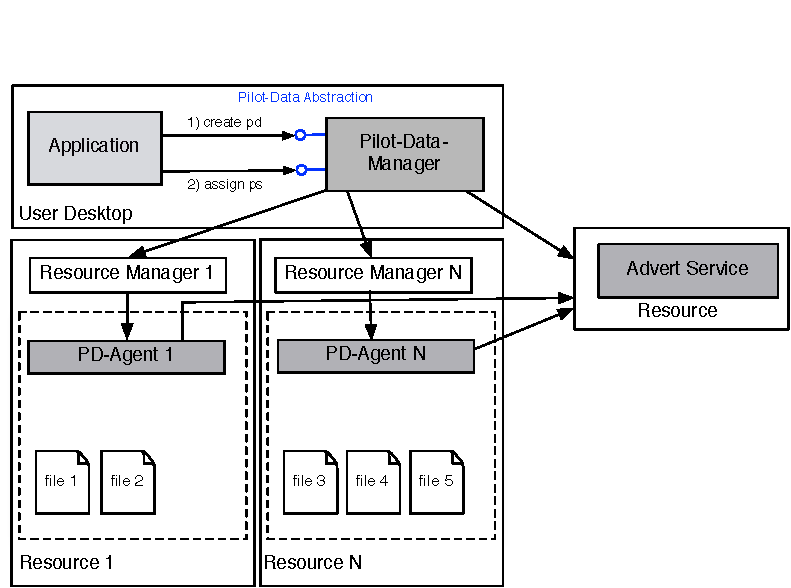
\includegraphics[width=0.48\textwidth]{figures/pilot-data-manager.pdf}
    \caption{\textbf{BigData Architecture:} The BD Manager exposes
      TROY's PD API. Application can create group of files and assign
      files to storage. The BD manager tracks file locations in the
      data catalog. The scheduler optimizes data-compute co-location.
      The transfer manager initiates and monitors data
      movements. \up\up}
    \label{fig:pilot-data-architecture}
\end{figure}

% \begin{figure*}[t]
%   \up\up\up
%   \begin{minipage}[t]{0.475\linewidth}
%     \centering
%     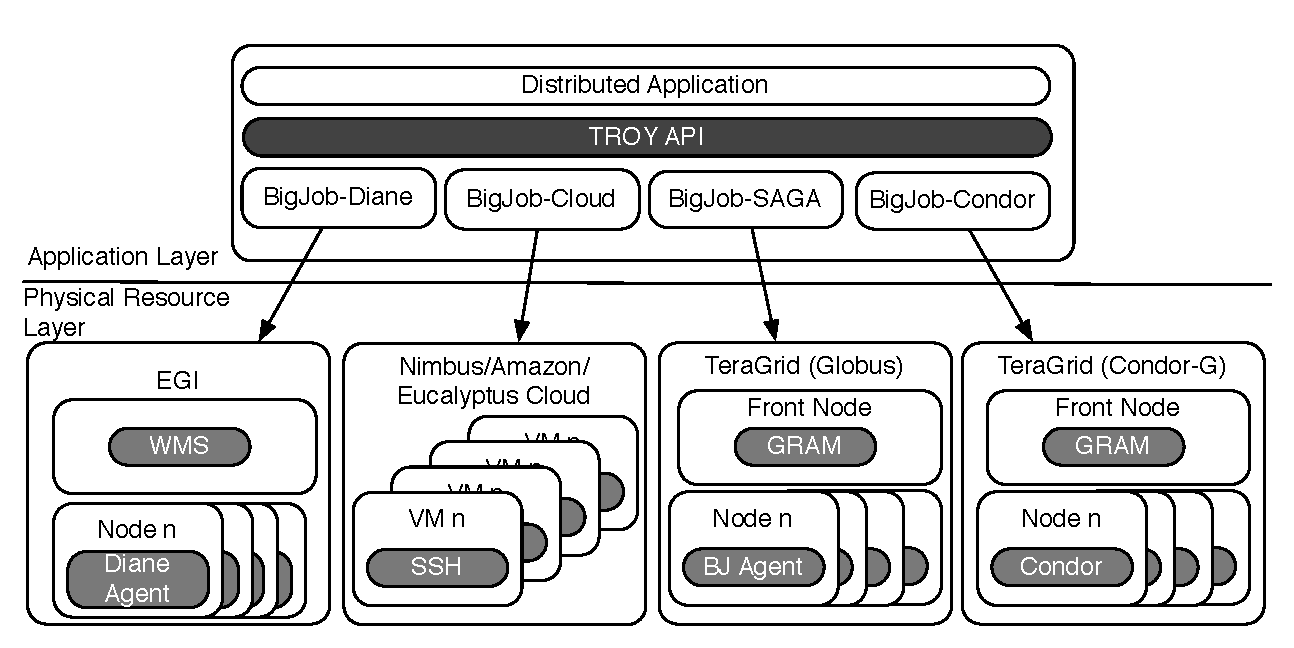
\includegraphics[width=\textwidth]{figures/distributed_pilot_job.pdf}
%     %\includegraphics[width=\textwidth]{figures/P1140340.JPG}
%     \caption{\textbf{BigJob -- SAGA-based Pilot-Job Implementation:}
%       BigJob is the implementation of the actual PJ functionality for
%       TROY. SAGA BigJob permits usage with multiple middleware
%       backends~\cite{}}
%     \label{fig:figures_distributed_pilot_job}
%     \end{minipage}
%   \hspace{0.035\linewidth}
%   \begin{minipage}[t]{0.475\linewidth}
%     \centering
%     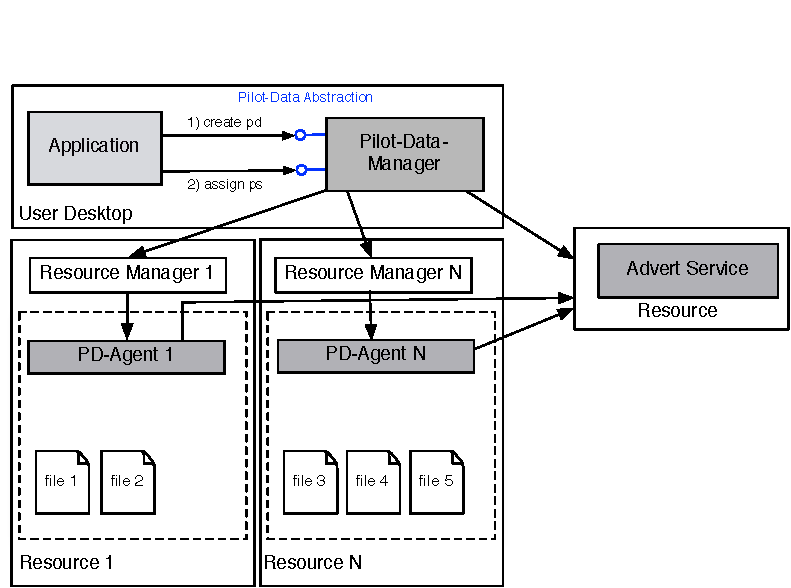
\includegraphics[width=\textwidth]{figures/pilot-data-manager.pdf}
%     \caption{\textbf{BigData Architecture:} The BD Manager exposes
%       TROY's PD API. Application can create group of files and assign 
%       files to storage. The BD manager tracks file locations in
%       the data catalog. The scheduler optimizes data-compute co-location.
%       The transfer manager initiates and monitors data movements. \up\up}
%     \label{fig:pilot-data-architecture}
%     \end{minipage}
% \end{figure*}

BigData-SAGA is the SAGA-based prototype of the Pilot-Data
abstraction; in the scope of this paper it is referred to as simply
BigData (BD).  Figure~\ref{fig:pilot-data-architecture} gives an
overview of the architecture.  The system consists of two components:
the BD manager, and the BD agents deployed on the physical
resources. The coordination scheme used is again M/W with some
intelligence that is located de-centrally at the BD agent. As
communication mechanism the SAGA Advert Service is used, in a similar
push/pull mode as for BJ.

The BD manager is responsible for 1) meta-data management, i.\,e.\ it
keeps track of the pilot stores that a pilot data object is associated
with, 2) for scheduling data movements and data replications (taking
into account the application requirements defined via affinities), and
3) for managing data movements activities.  Similar to BigJob, an
agent on each resource is used to manage the physical storage on a
resource.  

A particular critical requirement for data-intensive application, is
the management of affinity between DUs and also between WUs and
DUs. The BD scheduler supports preliminary affinity-aware
scheduling: both BigJob and BigData are tightly integrated to
efficiently support compute- and data-related aspects of dynamic
execution (see also \S{IIIA}).
 
\jhanote{Andre, please review the next paragraph: Should it just go
  for simplicity?} Thus, Pilot-Data introduces the PD container object
for expressing relationships between DUs. A PD corresponds to an SU in
the P* Model, i.\,e.\ it is used as scheduling unit for internal
optimizations, e.\,g.\ the grouping of DUs. Having instantiated a PD,
it can be assigned to a PS via the PD manager. A PS is a placeholder
reserving a certain amount of storage, i.\,e.\ it corresponds to a
pilot in the pilot-job model. By associating a PD to a PS the data is
actually moved to the physical location associated with the PS. The PD
manager facilitates the creation of PSs, schedules data movements
(with respect to specified affinities) and manages data accesses.


%%%%%%%%%%%%%%%%%%%%%%%%%%%%%%%%%%%%%%%%%%%%%%%%%%%%%%%%%%%%%%%%%%%%%%


% In addition to the three Pilot-Job framework discussed in this section, various
% other frameworks exist.
% \begin{itemize}
%     \item MyCluster~\cite{1652061} enables the 
% creation of a Condor, PBS or SGE clusters on-demand.
%     \item Falkon~\cite{1362680} is a Pilot-Job framework that emphasizes the 
% performance of its task dispatcher.
%     \item Nimrod/G~\cite{10.1109/HPC.2000.846563}
%     \item DIRAC~\cite{1742-6596-219-6-062049} is another pilot-job framework 
% used by the LHCb community.
%     \item ToPoS~\cite{topos} is a REST-based web service primarily designed with 
% respect to parameter sweep applications. Internally, ToPoS utilizes PJ 
% capabilities to efficiently manage resources.
%     \item The Production and Distributed Analysis System 
% (PanDA)~\cite{1742-6596-219-6-062041} is the workload management system of 
% the ATLAS experiment. PanDA utilizes multi-user PJs for resource management. 
% The PJ component is built on top of Condor-G and referred to as AutoPilot. 
% It can also be used independently of the ATLAS environment. 
% \end{itemize}


% 
% Both BigJob and BigData define similar elements that can be mapped to
% each other. Nevertheless, compute and data model sometimes require a
% different treatment.  The extended TROY (an implementation of the
% extended P* Model) will optimize data- and computing according to a
% set of defined affinities and policies.

% BJ and BD encapsulate cross-cutting properties across data and
% computation. 

% With the maturing of both models and
% implementations, we expect that both the PJ and PD model converge in
% the future.

\section{Discussion and Future Work \upp\upp}
\label{sec:discussion-future-work}

% The P* model was used to demonstrate
% We established PJ and PD as abstractions for supporting dynamic
% execution by decoupling workload and resource
% assignment/scheduling. 

% they share different important properties with respect to the commonly
% used communication and coordination schemes.

\alnote{Add discussion on limitations of API - address these
  limitations in a common runtime system.}

The primary intellectual contribution of this work has been the
development of the P* Model, the mapping of P* elements to PJ
frameworks such as DIANE and Condor-G, its validation via the
Pilot-API and demonstration of its use with multiple PJ frameworks.
 
The P* Model provides a common abstract model for describing and
characterizing Pilot-abstractions. We validate the P* Model by
demonstrating that the most widely used PJ frameworks, viz., DIANE and
Condor-G can be compared, contrasted and analyzed using this
analytical framework.

% , i.\,e.\ the architecture and the communication and coordination
% schemes.\alnote{i.e. sub-clause can go}

\jhanote{The Pilot-API captures the commonalities between the
  different PJ frameworks and provides a common access to them via a
  consistent API}.  Building on the P* Model, the Pilot-API's design
enables the easy exchange of PJ implementations, and also the
concurrent use of multiple PJ frameworks. The Pilot-API functions as
common access layer for different PJ frameworks, thus providing
interoperability and extensibility.

There is potential for immense practical implications of our work;
although these PJ frameworks collectively support millions of tasks
yearly on several production distributed infrastructure, extensibility
and interoperability remain significant challenges~\cite{extenci}.  As
alluded, many tools and frameworks were not engineered with
interoperability and extensibility as first-class considerations, and
are thus faced with real barriers. Given the increasing importance of
pilot-jobs and the challenges associated with distributed data
placement, our work which provides both a conceptual model and
practical solutions has the potential to ameliorate this situation.





\msnote{Need to introduce TROY now}
The TROY framework will be
extended to support advanced autonomic resource management and
selection strategies, e.\,g.\ by deploying more decentral decision
logic into the agents, thus providing possible further improvements to
scalability

% Having established the validity of the P* Model and TROY, in the
% future, 
%\alnote{this paragraph can IMHO be merged with the last paragraph}


Furthermore, our experience with fragile grid middleware and infrastructures
has taught us to appreciate the significance of details that come into play
while deploying software on heterogeneous distributed infrastructures, and which
in spite of theoretical and architectural advances have the potential to limit
impact. However, the SAGA inspired approach to the Pilot-API design and the
leverage of the design and deployment experiences of SAGA, e.\,g.\ by moving the
responsibility of correctly deployed grid-middleware to the resource providers
and not the end-users, should be an effective solution.
\amnote{last paragraph is somewhat hard to parse (first sentence).}

% Lack of interoperability also stems from the difference in the
% semantics; it is not wishful thinking that in addition to having a
% common and consistent API, PJ frameworks change their internal
% functioning to be make the consistent with the P* Model explicit.

\note{TROY provides a
  unified API that can be used to expose various PJ frameworks
  (e.\,g.\ BigJob, DIANE and Condor-G). Further, it enables the
  concurrent usage of multiple PJ frameworks (see
  figure~\ref{fig:figures_distributed_pilot_job}).  The SAGA inspired
  approach to TROY's API design --- its SAGA inspired adaptor-based
  architecture, leverage the design experiences of SAGA, are appealing
  to the pilot-job user community. Also, the chosen designs enables
  the easy exchange of PJ implementations and the concurrent use of
  multiple PJ frameworks. TROY thus functions as common access layer
  for different PJ frameworks, providing interoperability and
  portability of PJ applications. To some extent, the TROY API can be
  considered to be a prototype of a PJ-like API extension to SAGA (see
  Discussion \& future work, \S\ref{sec:discussion-future-work}).}

% \alnote{not sure about the capital letters in the (i) enumerations.
% We don't use this style anywhere else}

% i.e., PD and associated abstractions. However, only a prototype
% implementation of BigData exists;

P* provides significant future development, research \& deployment
extensions and opportunities. We discuss one opportunity along each of
these axes: (i) Development and Extension: In order to overcome
limitations of the API-based approach we will develop a complete
implementation of the P* -- called TROY (Tiered Resource Overlay)....
\jhanote{some details on TROY}. On the basis of successful validation
of the P* Model, we propose extensions to include data.  For example,
presenting unified abstractions within the Pilot-API and providing a
unified implementation of P* (e.g., BigData analagous to BigJob) in
(ii) Research Issues: These developments and extensions will also
provide the basis to explore and reason on the relative roles of
system versus application-level scheduling and heuristics for dynamic
execution; (iii) Deployment and Uptake: 
Currently..., % the widely used Condor-G
% framework is invoked via the Condor-SAGA adaptor; however, although
% the performance difference will be negligible, there will be
% significant ease of distribution if the Condor capabilities are
% directly integrated into TROY while retaining the advantage of a
% common consistent API to the PJ frameworks and functionality.
Additionally we aim to provide explicit support for advanced
dynamic execution modes and enhance the range of applications that
will benefit from the pilot abstraction. 

%\msnote{Not sure how iii fits in now}
% This
% should also result increased scalability.\alnote{not sure whether this is
% a significant scalability factor.}


In summary, we will use existing and emerging capabilities of TROY to
support the efficient and scalable solution of many scientific
applications that involve multiple independent tasks.\alnote{just one sentence - can be merged with paragraph above.}


\note{Future Work: TROY - tests on scalability and direct
  DIANE/Condor-G adaptors (more dev work) Claim BigData and BigJob
  into TROY and provide a unified Explore application with dynamic
  execution requirements: explore various kinds of dynamic execution
  and trade-offs }

% Without the advantages of scalability and extensibility arising from
% abstractions

% we propose a model for an
% abstraction of pilot-job frameworks.


% we will align the TROY API with the emerging SAGA Resource Management
% API~\cite{saga_rm}. We will further refine the TROY API, e.\,g.\ by
% generically supporting different security models via a context API
% (similar to the SAGA Context API).


%\note{work on scalability: Repex proposal?}

% \jhanote{Merge and Mix} Applications that support dynamic execution
% have the ability to respond to a fluctuating resource pool, i.\,e.,
% the set of resources utilized at time (T), $T=0$ is not the same as
% $T>0$. 


It is not possible to anticipate all of the tools and abstractions
that distributed applications will need down the road. Changes in
infrastructure and application requirements cannot be predicted. For
this reason, tools must provide open interfaces to enable more easy
integration and interoperation with other tools. Whether this can be
best achieved by new extensible tools or “tool orchestration” or a
tool “framework” is an open question. This, of course, does not
preclude the internal evolution of existing tools to implement new
abstractions, but just this is not enough in our view.

% Distributed applications that have been able to break the coupling
% between workload management and resource assignment/scheduling have
% been successful at efficiently utilizing distributed resources..





\up
\section*{Acknowledgements\upp\upp}
\footnotesize{This work is funded by NSF CHE-1125332 (Cyber-enabled
  Discovery and Innovation), HPCOPS NSF-OCI 0710874 award, NSF-ExTENCI
  (OCI-1007115) and NIH Grant Number P20RR016456 from the NIH National
  Center For Research Resources. Important funding for SAGA has been
  provided by the UK EPSRC grant number GR/D0766171/1 (via OMII-UK)
  and the Cybertools project (http://cybertools .loni.org; PI Jha)
  NSF/LEQSF (2007-10)-CyberRII-01. SJ acknowledges the e-Science
  Institute, Edinburgh for supporting the research
  theme. ``Distributed Programming Abstractions'' \& 3DPAS. We thank J
  Kim (CCT) for assistance with the DNA models.  MS is sponsored by
  the program of BiG Grid, the Dutch e-Science Grid, which is
  financially supported by the Netherlands Organisation for Scientific
  Research, NWO. SJ acknowledges useful related discussions with Jon
  Weissman (Minnesota) and Dan Katz (Chicago). This work has also been
  made possible thanks to computer resources provided by TeraGrid TRAC
  award TG-MCB090174 (Jha). This document was developed with support
  from the National Science Foundation (NSF) under Grant No.  0910812
  to Indiana University for ``FutureGrid: An Experimental,
  High-Performance Grid Test-bed''.}  \up
%\bibliographystyle{plain}
\bibliographystyle{IEEEtran}
\bibliography{pilotjob,saga,saga-related}
\end{document}


\note{Facilities provided include the creation of a PJ, insertion of
  tasks, and attachment to a CPU resource pool for late-binding task
  execution.}  \note{Tasks are ultimately loaded onto specific
  resources using the pilot-job and late-binding. In other words}
\note{PJ provides a mechanism to decouple “task coordination” from
  “resource mapping”.}




% To perform the above experiments we built an application \smnote{this
% application is DARE. do we need mention it here?} using TROY API to submit Bfast
% \cu 's with different input files to different backend implementations. The \cu 's
% are completely handled and submitted to different backends by TROY and the
% co-ordination of \cu 's was made simple for the application. Further, applications
% can also continuously monitor status of remote agents and UOWs.

% Further, it shows that both PJ implementations can be used
% concurrently. This is particularly useful if the time-to-completion can be
% reduced in cases where resources on another infrastructure are available.





% Figure~\ref{fig:perf_perf-bfast-bj} shows the results of the
% experiments. The time-to-completion for TROY-DIANE is about 207\,sec
% longer than for TROY-SAGA. The main contributor for this increased
% runtime is the deployment time required for DIANE. In a multi-node
% setup multiple work agents must be used (8 in this case).  For each
% worker agent DIANE must be downloaded, installed and started
% separately. In total this requires about 178\,sec. Further, each DIANE
% worker agent is queued as a separate job at the local resource manager
% -- this contributes the the higher deviation in the measured
% runtimes. Because BigJob requires a pre-run installation on each site,
% it only shows a startup time of 28\,sec. Additionally, we also
% observed a runtime overhead of about 17\,sec for the TROY-DIANE
% scenario. This overhead is likely caused by the additional agents
% required.

% % In the case of BJ-DIANE backend Multinode submitter was not used/not % yet. As
% a result it submits job request's for each node separately and there % also some
% delay between actual launch and startup time of UOW. Further, DIANE % was
% installed separately for every agent/node requested.

% \alnote{commented out for submission: A reflection on the Reality of Distributed Infrastructures}

%\subsection{A reflection on the Reality of Distributed Infrastructures}



% Further, TROY hides many of the complications with various pilot
% jobs like multiple node backend agents, how \cu 's distribution to
% various backends. Thus, this enables users of this API to
% concentrate more on designing their applications instead worrying
% about the various configurations of the pilot jobs.

However, even for traditional
high-performance/parallel applications, the evolution or internal
dynamics of an application may vary, thereby changing the resource
requirements.  For example, different solvers, adaptive algorithms
and/or implementations, can also require applications to utilize
different set/amounts of resources.  Thus, the need to support dynamic
execution is widespread for computational science applications.

% PJ provide a simple model for distributed resource usage.
% Pilot-jobs enable this decoupling typically in user-space without the
% policy-level complexity of implementing advanced reservations. 

%Pilot-jobs typically in user-space (i.e. application-level
%scheduling).  

%Although there are many implementations of the PJ abstraction

% , and are, in general, expensive to develop and manage in terms of
% the time and effort involved.  T Tools tend to be customized to
% specific applications and their requirements, with limited concern
% for reuse or extensibility. For example de- spite community efforts
% such as CCA, few applications, if any, mix-and-match components
% developed by different projects.

% In fact, not only do distributed applications need abstractions to
% support the requirements through the individual stages of
% development, deployment and execution, support for applications
% through these stages needs to be a coherent integrated activity, as
% opposed to a disjointed effort..  There are just too many moving
% parts!
% pilot-data % (PD) 

% to treat data as a first-class schedulable entity, is a concept
% analogous to PJ:

%  We present and discuss
% the P* model in \S{II}.


% Both PJ/PD frameworks rely on SAGA for implementation
% of the actual PJ/PD functionality. 
% Using the adaptor mechanism, TROY
% can further be extended to other PJ implementations.

% \jhanote{Note the distinction between pilot-jobs and pilot-job
%   framework: DIANE, Swift are PJ frameworks. Specific instances of
%   these tools/usage give rise to pilot-jobs.}\alnote{added PJ
%   framework definition to terms and usage.}

% which exposes
% the semantics of PJs in a P* conform way, and a runtime
% environment. 
% \alnote{OLD: As we will discuss, consistent with the goals and aims of
%   SAGA, there can be multiple instances of BigJob for different
%   backends.}\jhanote{Have we not gone to multiple instances of the
%   Pilot-Job for TROY and not multiple instances of
%   BigJob?}\alnote{refined}
% and outline briefly how other well known pilot-jobs can be
% understood using the {\it vectors}~\cite{dpa_surveypaper} of the P*
% Model.
% \alnote{do we validate just the TROY API or the TROY framework?}



% \jhanote{Should we to introduce Dynamic Applications explicitly in the
%   title? Just a question, not a suggestion...}

%\subsection{Introduction \jhanote{SJ, AL}}


%\section{Pilot-* : An abstraction for Dynamic Execution}
%\section{TROY: A Model of Pilot-Abstractions for Dynamic Execution}



% Figure~\ref{fig:figures_pstar}
% illustrates the interactions between the elements of the P*
% model. Although there can be variations, a typical usage scenario
% consists of the following steps: The application specifies the
% capabilities of the resources required (step 1).  \jhanote{Andre,
%   Mark: Is Step 1 true? Couldn't we just say: application specifies
%   the \cu ?} During the instantiation of a PJ and the assignment of
% resources to the PJ, pilots are queued and started via the local
% resource manager (step 1-4).
% 
% \jhanote{We should talk about ``API'' --- \cu  crossing P* API, ie
%   controlled by Pilot-Manager, and then becoming an SU thereafter.
%   Also talk about multi-level scheduling. Anything that focusses the
%   reader's attention on an understanding that was not covered in brief
%   description} \alnote{refined}
% 
% Commonly, the pilot-manager (PM) can be accessed via a set of command
% line tools and/or an API via which an application can create and
% submit \cus to the pilot-manager (step 5/6). A \cu  that is submitted
% becomes a SU, i.\,e.\ the PM is now in control of it and schedules and
% manages its execution. In the simplest case one \cu  corresponds to one
% SU; however, SUs can be combined and aggregated to optimize
% throughputs and response times.
% 
% Commonly, a hierarchical M/W coordination model is used: On
% the first level, the PM uses M/W in order to coordinate the actions of
% the pilots that are part of its resource pool (usually 1 or
% more). Once a SU is forwarded to a pilot, the pilot is responsible for
% the coordination of the SU execution. Again a pilot usually manages 1
% or more SUs using M/W. \jhanote{Need some clarification: what is the
%   worker/agent here? (i) Isn't it PJ Frameworks that use M-W
%   coordination and not the PJ.  Also, in the framework, isn't the
%   Manager the Master, and the Pilot-Job the Worker; What about \cu /SU ?
%   ie if \cu /SU are the workers, what is the master?}  \alnote{refined}
% Scheduling decisions can be conducted on each level. The delegation of
% decision capabilities into lower levels, i.\,e.\ the pilot, can yield
% to a more autonomic and adaptive behavior as well as a better
% scalability.
% 
% \alnote{TODO: remove redundancy with paragraph above} As explained, a
% P* implementation usually operates a hierarchy of schedulers.  The
% following examples involves a two-level hierarchy: In the first
% hierarchy level the PM schedules an SU to a pilot of its resource pool
% (step 7). Another round of scheduling can occur within the pilot,
% i.\,e.\ the pilot decides when and on what physical resource a SU is
% executed (step 8). Further, the pilot manages the subsequent execution
% of the SU on the physical resource on which the pilot is operating.



% \jhanote{Integrate.. next sentence} PJ frameworks with decentralized
% decision often utilize autonomic agents that accepts respectively pull
% SUs according to a set of defined policies.


% \alnote{We use the term agent to denote a component inside the pilot
%   that has some decision making capability. In most cases we could
%   replace agent just with pilot. However, when talking about decentral
%   coordination with autonomic decision making this will be
%   difficult. Should we explicitly define an agent in sec II under
%   Pilot-Job (aka pilot)?}
 


%or the implementation of a custom scheduler is supported.
% \jhanote{Move to an appropriate location}\jwave{Commonly }
% \jhanote{Mention that application/user level input/heuristics can be
%   employed at either of the two stages: binding and/or scheduling}
% \jhanote{Candidate for removal}\jwave{Furthermore, the time of binding
%   influences the point at which the binding decision is made, e.\,g.\
%   in the case of early binding, the decision could be made by the
%   application, while in late binding mode the decision is made by the
%   PJ framework.}
% \jhanote{Integrate: Note that that this can either be a simple
%   grouping or a smart aggregation of \cus (e.\,g.\ two sets of
%   parameters merged into one).}
